\chapter{二分类学习的可学习性}
\label{chap:binary-learnability}

第~\ref{chap:statistical-learning-framework}章的垃圾邮件例子中，阈值0.4和0.6都判对了四封训练邮件，却对分数落在0.4与0.6之间的邮件给出相反的判断。训练样本无法区分这两个假设，而在这些邮件上，二者至少有一个会出错。如果再多抽一些邮件，就有机会抽到分数落在这个区间的邮件，从而看出哪个阈值出错。本章研究这件事的定量形式：训练样本要有多少，才能保证学习算法依据样本选出的假设，在新邮件上的错误率也低。

我们先建立直觉。设某个假设在全部邮件上的错误率较高，称它为坏假设。随机抽取一封邮件时，它有一定概率在这封邮件上出错；抽取的邮件越多，它恰好判对每一封训练邮件的概率就越小。如果只需检验一个事先选定的假设，这个概率已经足以说明样本量的作用。然而，学习算法是看过样本之后才从假设空间中挑选假设的：只要某个坏假设恰好判对了全部训练邮件，算法就可能选中它。因此需要保证的是，假设空间中没有任何坏假设能在训练样本上表现得和好假设一样。假设空间越大，出现这种例外的机会越多，所需的样本也越多。样本量分析由此要同时考虑两个量：单个坏假设在训练样本上不被识别出来的概率，以及假设空间的大小。

本章的路线由“怎样衡量假设空间的大小”这个问题串起来。假设只有有限个时，假设个数就是合适的度量（第~\ref{sec:binary-finite-class}、\ref{sec:binary-uniform-convergence}节）。实数阈值这类空间含有无穷多个假设，个数失去意义；第~\ref{sec:binary-infinite-class}节改为统计假设在有限个输入上能给出多少种不同的预测，由此得到一个新的度量，并证明在本章条件下它有限恰好等价于可学习。这个度量按最不利的输入位置计算，不看实际抽到的样本；第~\ref{sec:rademacher-complexity}节改在已抽到的样本上衡量函数类，得到可由数据估计的风险上界。随后两节换两个角度：输出能否由少量训练样本重新构造出来（第~\ref{sec:sample-compression}节），以及由多个假设组合成的输出如何分析（第~\ref{sec:boosting}节）。最后，第~\ref{sec:computable-binary-learning}节检查样本量存在之后，训练和预测能否由程序在有限时间、可接受的资源内完成。

全章沿用第~\ref{sec:learning-problem}节的二分类设定：每条观测由输入和取值为0或1的标签组成，训练样本独立同分布；预测错误计损失1，预测正确计损失0，即零一损失。学习成功的标准是第~\ref{sec:pac-learning}节的可实现PAC和不可知PAC。各节的区别在于用什么量衡量假设空间的复杂度，以及怎样控制“先看样本、再选假设”带来的偏差。除非另行说明，比较决策空间取为假设空间$\mathcal H$，学习算法也从$\mathcal H$中输出假设；样本压缩、集成学习和可计算PAC学习三节允许输出$\mathcal H$以外的分类器，即非恰当学习，届时会注明。

\section{可实现的有限假设空间}
\label{sec:binary-finite-class}

先考虑最简单的情形：假设空间只包含有限个假设。仍以垃圾邮件过滤为例，假定学习算法只能在0.2、0.4、0.6、0.8这四个阈值中选择，分数不低于阈值的邮件判为垃圾邮件。邮件分数仍可以是$[0,1]$中的任意值，受到限制的只是可供选择的判定规则，于是假设空间只含四个假设。对于有限个假设，我们可以分别计算每个坏假设在训练样本上全部判对的概率，再把这些概率相加，得到“至少有一个坏假设全部判对”的概率上界。

本节先讨论可实现情形，即假设空间中存在一个总体风险为零的假设$h^\star$。总体风险为零表示$h^\star$出错的概率为零，因此它在训练样本上几乎必然不犯错，经验风险最小化（ERM）选出的假设在训练样本上的错误数也就为零。训练错误为零的假设称为与样本\term{一致}（consistent）。一致只说明这个假设判对了当前样本中的全部标签，并不说明它在未见过的输入上也判对。

一致的假设仍可能有较高的总体风险。设某个阈值在全部邮件上的错误率为20\%，它判对一封随机邮件的概率就是80\%。训练样本中的$n$封邮件独立抽取，它判对全部$n$封的概率为$0.8^n$。$n=10$时，这个概率约为0.11，并不小；一旦发生，这个阈值在训练样本上与零风险的$h^\star$一样没有错误，只看样本的ERM无法区分二者，可能选中它。$n$增大时$0.8^n$迅速减小，但ERM面对的高风险假设不止一个，所以要控制的是：假设空间中存在某个高风险假设与样本一致的概率。

下面把20\%换成任意给定的容限$\varepsilon$，把总体风险超过$\varepsilon$的假设称为高风险假设。记$Y=\{0,1\}$，训练样本$S\sim\mathcal P^n$。先在抽样之前固定一个假设$h\in\mathcal H$。若$R_{\mathcal P}(h)>\varepsilon$，它判对一条随机观测的概率小于$1-\varepsilon$；由于各条观测独立，它判对全部$n$条观测的概率等于各条概率之积：
\begin{equation}
  \mathbb P\bigl(\hat R_S(h)=0\bigr)
  =\bigl(1-R_{\mathcal P}(h)\bigr)^n
  \leq(1-\varepsilon)^n\leq e^{-n\varepsilon}.
  \label{eq:bad-consistent-hypothesis}
\end{equation}
式~\eqref{eq:bad-consistent-hypothesis}只适用于抽样之前固定的假设，而ERM的输出依赖于样本，不能直接代入。为此考察一个范围更大的事件：假设空间中至少有一个高风险假设与样本一致。如果ERM输出了高风险假设，这个输出本身与样本一致，上述事件必然发生；所以只要控制这个事件的概率，就控制了ERM失败的概率。这个事件是各个高风险假设“与样本一致”事件的并集，由并集界，它的概率不超过各事件概率之和。并集界不要求事件互斥，多个假设同时与样本一致并不影响结论。有限假设空间中至多有$|\mathcal H|$个高风险假设，由此得到下面的样本量界。

\begin{theorem}[有限假设空间的可实现PAC样本量界]
\label{thm:finite-realizable-pac}
设$(X,\mathcal X)$为可测空间，$Y=\{0,1\}$取离散$\sigma$代数，
$\mathcal H\subseteq Y^X$是由可测分类器组成的非空有限集合，$\mathcal P$是
$X\times Y$上的联合分布。采用零一损失，并记
\[
 R_{\mathcal P}(h)=\mathbb P_{(x,y)\sim\mathcal P}\{h(x)\neq y\},\qquad
 \hat R_S(h)=\frac1n\sum_{i=1}^n\mathbb I\{h(x_i)\neq y_i\}.
\]
设$n\geq1$、$S=((x_i,y_i))_{i=1}^n\sim\mathcal P^n$，且存在
$h^\star\in\mathcal H$满足$R_{\mathcal P}(h^\star)=0$。对任意
$\varepsilon,\delta\in(0,1)$，若可测学习算法（允许内部随机性）以概率1输出满足
$\hat R_S(\hat h)=0$的$\hat h\in\mathcal H$，则
\begin{equation}
  \mathbb P_{S,A}\bigl(R_{\mathcal P}(\hat h)>\varepsilon\bigr)
  \leq |\mathcal H|e^{-n\varepsilon}.
  \label{eq:finite-realizable-failure}
\end{equation}
特别地，只要
\begin{equation}
  n\geq\frac{\log|\mathcal H|+\log(1/\delta)}{\varepsilon},
  \label{eq:finite-realizable-sample}
\end{equation}
算法就以至少$1-\delta$的概率输出期望风险不超过$\varepsilon$的假设；这里的概率
同时来自$S\sim\mathcal P^n$和算法的内部随机性。
\end{theorem}

\begin{proof}
题设保证输出几乎必然与样本一致；可实现性也使这样的选解存在。输出风险若超过$\varepsilon$，至少一个高风险假设与全部观测一致。由此
\begin{align*}
 \mathbb P\bigl(R_{\mathcal P}(\hat h)>\varepsilon\bigr)
 &\leq \mathbb P\bigl(\exists h\in\mathcal H:
       R_{\mathcal P}(h)>\varepsilon,\ \hat R_S(h)=0\bigr)\\
 &\leq\sum_{h:R_{\mathcal P}(h)>\varepsilon}
       \mathbb P\bigl(\hat R_S(h)=0\bigr)
 \leq |\mathcal H|e^{-n\varepsilon}.
\end{align*}
将末项限制为$\delta$并解出$n$，即得式~\eqref{eq:finite-realizable-sample}。
\end{proof}

把四阈值的例子代入式~\eqref{eq:finite-realizable-sample}。设四个阈值中有一个总体风险为零，要求以至少99\%的概率得到总体风险不超过5\%的假设，即$\delta=0.01$、$\varepsilon=0.05$。式~\eqref{eq:finite-realizable-sample}给出充分样本量$\lceil(\log4+\log100)/0.05\rceil=120$。这个样本量不依赖于邮件分数和标签的具体分布：只要分布满足可实现条件，独立抽取120封邮件后，任何输出一致假设的算法都满足上述要求。它是充分条件；定理并没有说少于120封就一定达不到。

若可选阈值增加到8个，容限和置信水平不变，充分样本量变为$\lceil(\log8+\log100)/0.05\rceil=134$。假设个数加倍，取整前的样本量只增加$\log2/\varepsilon\approx13.9$，因为假设个数在式中以对数形式出现。更一般地，对任意有限假设空间和任意$\varepsilon,\delta$，式~\eqref{eq:finite-realizable-sample}都给出一个不依赖分布的样本量，所以有限假设空间是可实现PAC可学习的。这一结论只涉及样本量；从有限空间中找出一致假设需要多少计算，留到第~\ref{sec:computable-binary-learning}节讨论。

上述论证依赖可实现性：零风险假设的存在保证ERM能够选出一致假设，于是只需排除“高风险假设也与样本一致”这一种情况。若标签带有噪声，例如一部分邮件被人工误标，假设空间中可能没有任何假设能判对全部训练邮件，ERM比较的就不再是“有没有出错”，而是各假设出错比例的高低。这时，总体风险较高的假设可能恰好在这份样本上错得较少，从而被ERM选中。要排除这种情况，需要样本上的错误比例足够接近总体风险，训练样本上的比较结果才能反映总体风险的高低。下一节讨论这一要求。

\section{不可知的有限假设空间}
\label{sec:binary-uniform-convergence}

不可知情形下，假设空间中不一定存在零风险假设，学习的目标是使输出的总体风险接近$\mathcal H$中的最低水平。ERM依据经验风险比较假设，要让这种比较可靠，一个充分的办法是要求同一份样本把所有假设的总体风险都估计准确。这样，无论ERM看过样本后选出哪个假设，它的经验风险都接近总体风险；用来作比较的任一参照假设也是如此，于是样本上的比较结果可以转移到总体风险上。同一份样本同时把所有假设的风险估计准确，这一性质称为一致收敛，正式定义稍后给出。对有限假设空间，可以先分别估计每个假设偏差过大的概率，再把这些概率相加；对无限假设空间，相加的项数没有上限，第~\ref{sec:binary-infinite-class}节将改为统计预测模式。

先看一个在抽样前固定的假设$h$，例如事先选定的某个阈值。抽到的样本不同，$h$的经验风险也不同。每条观测上的零一损失取值0或1，均值为$R_{\mathcal P}(h)$；$n$条观测的损失相互独立，所以经验风险是$n$个独立Bernoulli随机变量的平均。Hoeffding不等式说的是：独立且取值有界的随机变量，其平均值偏离均值的概率随样本量指数下降，下降速度只取决于取值区间的长度，不需要知道分布的其他信息。对取值于$[0,1]$的损失，它给出偏离超过$\eta$的概率上界（证明可参考\BookVolumeRef{vol:mathematical-preliminaries-lower}{卷2《数学准备：概率、因果与决策》}）：
\begin{equation}
 \mathbb P\left(\left|\hat R_S(h)-R_{\mathcal P}(h)\right|>\eta\right)
 \leq2e^{-2n\eta^2}.
 \label{eq:hoeffding-fixed-hypothesis}
\end{equation}
式~\eqref{eq:hoeffding-fixed-hypothesis}同样只适用于抽样前固定的假设，不能直接用于依赖样本的输出$A(S)$。以四个阈值为例，ERM计算四个经验风险并选出最小者。若只保证其中某一个阈值的风险估计准确，ERM选出的可能恰好是另一个经验风险被低估的阈值。反过来，若四个阈值的偏差都不超过$\eta$，ERM输出的总体风险至多比四者中的最低总体风险高$2\eta$：从输出的总体风险换到它的经验风险，误差至多$\eta$；输出的经验风险不高于最优阈值的经验风险；再从后者换回最优阈值的总体风险，误差又至多$\eta$。定理~\ref{thm:finite-agnostic-pac}的证明会写出这三步。图~\ref{fig:learning-uniform-convergence}中，每条竖线表示一个假设的经验风险与总体风险之差；只有全部竖线都短，ERM依据样本选出的输出才一定受到控制。

\begin{figure}[htbp]
  \centering
  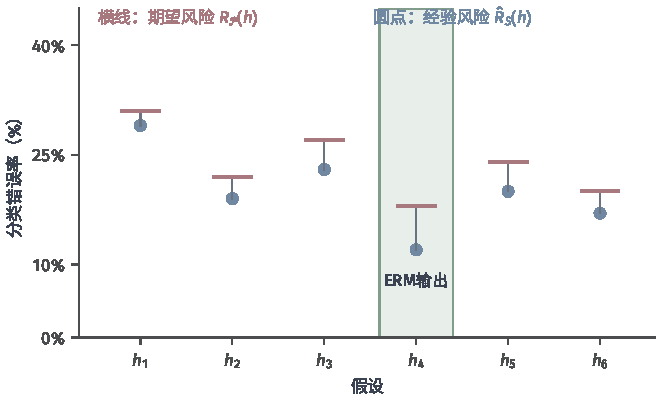
\includegraphics[width=112.000mm]{figures/03-foundations/02-learning-theory/matplotlib/learning-theory-uniform-convergence/figure.pdf}
  \caption{单个风险估计与共同保证。竖线连接各假设的经验风险与期望风险；只限制其中一条线，不能覆盖ERM在框中选择的输出。限制全部竖线后，这个数据依赖输出也落在保证内。}
  \label{fig:learning-uniform-convergence}
\end{figure}

因此我们需要这样一种保证：对给定的偏差容限$\eta$和失败概率$\delta$，存在一个样本量，独立抽取这么多观测后，以至少$1-\delta$的概率，所有假设的偏差都不超过$\eta$；并且这个样本量不能依赖未知的分布。下面先说明正式定义所需的技术约定，再写出这一要求。

\paragraph{可测性与可分性约定}

正式条件涉及“所有假设偏差的上确界”这一随机变量，只有它可测，相应的概率才有定义。对有限空间，这个上确界是有限个可测随机变量的最大值，因而可测。对无限空间，上确界要取遍下面的零一损失函数类，可测性不再自动成立：
\[
 \mathcal F_{01}=\{(x,y)\mapsto\ell_{01}(h(x),y):h\in\mathcal H\}
\]
为避免这一技术困难，本章沿用第~\ref{sec:learning-problem}节的可测性与可分性约定，保证相关的上确界和比较事件可测；后文的压缩映射、重构映射和学习器等依赖样本的映射也都要求可测。可实现情形下，学习算法选取与样本一致的假设；其他需要证明学习器存在的地方，使用该约定给出的可测近似ERM。缺少这些技术条件时，下面的结论不能直接套用。

% 保留旧位置锚点，不再重复编号定义。
\phantomsection\label{def:learning-uniform-convergence}
据此，对零一损失类$\mathcal F_{01}$定义\term{一致收敛}（uniform convergence）：同一份样本要以高概率同时把所有假设的风险估计准确，并且所需样本量对所有允许的联合分布统一适用。具体地，对任意$\eta,\delta\in(0,1)$，存在一个只依赖于$\mathcal H,\eta,\delta$的样本量$m_{\mathcal H}^{\mathrm{UC}}(\eta,\delta)$，使得在可测性与可分性约定下，对任意联合分布$\mathcal P$和任意$n\geq m_{\mathcal H}^{\mathrm{UC}}(\eta,\delta)$，都有
\begin{equation}
 \mathbb P_{S\sim\mathcal P^n}\left(
   \sup_{h\in\mathcal H}|\hat R_S(h)-R_{\mathcal P}(h)|\leq\eta
 \right)\geq1-\delta.
 \label{eq:learning-uniform-convergence-definition}
\end{equation}

式~\eqref{eq:learning-uniform-convergence-definition}中的上确界取遍$\mathcal H$中所有假设的偏差；它不超过$\eta$，就意味着每个假设在这份样本上的偏差都不超过$\eta$，上确界本身不必由某个假设取到。概率保证允许偶尔抽到偏差较大的样本，只要这种样本出现的概率不超过$\delta$。这里的$\mathcal P$是输入与标签的联合分布，既描述各种邮件出现的频率，也描述给定输入时标签如何取值。不同分布下各假设的总体风险不同，但样本量$m_{\mathcal H}^{\mathrm{UC}}(\eta,\delta)$必须对所有分布同时适用。一致收敛不要求存在零风险假设，所以它适用于不可知设定，所覆盖的分布与定义~\ref{def:general-pac-learnability}相同。

一致收敛要求的是风险估计准确，并不要求风险小。一个总体风险为40\%的假设，只要它在样本上的错误比例也接近40\%，就满足一致收敛的要求；从中选出风险小的假设，是一致收敛成立之后由ERM完成的事。

对有限空间，“所有偏差都不超过$\eta$”的反面是“至少一个假设的偏差超过$\eta$”。式~\eqref{eq:hoeffding-fixed-hypothesis}给出单个假设偏差超过$\eta$的概率，对有限个假设应用并集界，就得到后一事件的概率上界，从而得到下面的定理。

\begin{theorem}[有限假设空间的一致收敛样本量界]
\label{thm:finite-uniform-convergence}
设$(X,\mathcal X)$为可测空间，$Y=\{0,1\}$取离散$\sigma$代数，
$\mathcal H\subseteq Y^X$是由可测分类器组成的非空有限集合，$\mathcal P$是
$X\times Y$上的任意联合分布。对零一损失，记
\[
 R_{\mathcal P}(h)=\mathbb P_{(x,y)\sim\mathcal P}\{h(x)\neq y\},\qquad
 \hat R_S(h)=\frac1n\sum_{i=1}^n\mathbb I\{h(x_i)\neq y_i\}.
\]
设$n\geq1$且$S=((x_i,y_i))_{i=1}^n\sim\mathcal P^n$。对任意
$\eta,\delta\in(0,1)$，只要样本量满足
\begin{equation}
 n\geq\frac{\log(2|\mathcal H|/\delta)}{2\eta^2},
 \label{eq:finite-uniform-sample}
\end{equation}
就有
\[
 \mathbb P_{S\sim\mathcal P^n}\left(
 \sup_{h\in\mathcal H}|\hat R_S(h)-R_{\mathcal P}(h)|\leq\eta
 \right)\geq1-\delta.
\]
同一概率界也可写为：对任意$n\geq1$和$\delta\in(0,1)$，以下不等式以至少$1-\delta$的概率成立：
\begin{equation}
 \sup_{h\in\mathcal H}|\hat R_S(h)-R_{\mathcal P}(h)|
 \leq\sqrt{\frac{\log(2|\mathcal H|/\delta)}{2n}}.
 \label{eq:finite-uniform-bound}
\end{equation}
由于该样本量不依赖$\mathcal P$，有限假设空间满足分布无关的一致收敛。
\end{theorem}

\begin{proof}
对每个$h$使用式~\eqref{eq:hoeffding-fixed-hypothesis}。上确界超过$\eta$等价于至少一个假设的偏差超过$\eta$；对这些事件求并集界，得到
\[
 \mathbb P\left(\sup_{h\in\mathcal H}|\hat R_S(h)-R_{\mathcal P}(h)|>\eta\right)
 \leq 2|\mathcal H|e^{-2n\eta^2}.
\]
按式~\eqref{eq:finite-uniform-sample}选择$n$使右侧至多为$\delta$；或令右侧等于$\delta$，反解偏差$\eta$，得到式~\eqref{eq:finite-uniform-bound}。两种写法的样本要求均与具体$\mathcal P$无关。
\end{proof}

一致收敛给出了“所有假设同时估计准确”的事件。在这个事件上，ERM输出$\hat h$的经验风险不高于任一参照假设$h\in\mathcal H$的经验风险；把两边的经验风险分别换成总体风险，各产生至多一个偏差，就得到输出与参照的总体风险之差的上界。下面据此给出有限空间在不可知情形下的样本量。

\begin{theorem}[有限假设空间的不可知PAC样本量界]
\label{thm:finite-agnostic-pac}
设$(X,\mathcal X)$为可测空间，$Y=\{0,1\}$取离散$\sigma$代数，
$\mathcal H\subseteq Y^X$是由可测分类器组成的非空有限集合，$\mathcal P$是
$X\times Y$上的任意联合分布。对零一损失，记
\[
 R_{\mathcal P}(h)=\mathbb P_{(x,y)\sim\mathcal P}\{h(x)\neq y\},\qquad
 \hat R_S(h)=\frac1n\sum_{i=1}^n\mathbb I\{h(x_i)\neq y_i\}.
\]
设$n\geq1$、$S=((x_i,y_i))_{i=1}^n\sim\mathcal P^n$，可测学习算法
$A$（允许内部随机性）以概率1输出
$\hat h=A(S)\in\argmin_{h\in\mathcal H}\hat R_S(h)$。对任意
$\varepsilon,\delta\in(0,1)$，只要
\begin{equation}
 n\geq\frac{2}{\varepsilon^2}
 \left(\log(2|\mathcal H|)+\log\frac1\delta\right),
 \label{eq:finite-agnostic-sample}
\end{equation}
就有
\[
 \mathbb P_{S,A}\left(
 R_{\mathcal P}(\hat h)\leq\inf_{h\in\mathcal H}R_{\mathcal P}(h)+\varepsilon
 \right)\geq1-\delta.
\]
概率同时来自样本抽取和$A$的内部随机性。
\end{theorem}

\begin{proof}
在定理~\ref{thm:finite-uniform-convergence}中将容限设为$\eta=\varepsilon/2$。式~\eqref{eq:finite-agnostic-sample}使全部风险偏差不超过这个容限的概率至少为$1-\delta$。固定满足条件的样本，再取任意$h\in\mathcal H$；输出$\hat h$也在该空间内，两者均受偏差界约束。结合ERM的经验最优性，有
\begin{align*}
 R_{\mathcal P}(\hat h)
 &\leq\hat R_S(\hat h)+\frac{\varepsilon}{2}\\
 &\leq\hat R_S(h)+\frac{\varepsilon}{2}\\
 &\leq R_{\mathcal P}(h)+\varepsilon.
\end{align*}
首尾两次比较分别连接输出和参照的经验风险与总体风险，中间一次使用ERM。结论对任意$h$成立，取下确界即得所需保证。
\end{proof}

这个定理控制的是输出的总体风险比$\mathcal H$中最低总体风险高出多少。与可实现情形相比，样本量对精度的依赖从$1/\varepsilon$变成了$1/\varepsilon^2$，原因在于两种情形要排除的事件不同。可实现情形只需排除“某个高风险假设在全部样本上都不出错”，对固定假设，这个概率按$e^{-n\varepsilon}$随$n$下降。不可知情形下，各假设通常都会出错，沿本节的一致收敛充分路线比较它们的错误比例时，我们把每个总体与经验错误率之差统一控制在$\varepsilon/2$以内；Hoeffding不等式给出的偏差概率为$e^{-2n\eta^2}$，取$\eta=\varepsilon/2$后需要$n\varepsilon^2$足够大，因此样本量按$1/\varepsilon^2$增长。这一差别来自分析中需要控制的事件不同。

同一个偏差界还可以用来给出第~\ref{sec:statistical-model-selection}节结构风险最小化（SRM）中的惩罚项（定理~\ref{thm:srm-oracle-bound}）。设事先给定一列嵌套的有限假设空间$\mathcal H_1\subseteq\mathcal H_2\subseteq\cdots$。SRM在看过样本之后才选择空间编号$k$和其中的假设$h$。如果只保证某个事先选定的空间内估计准确，SRM可能转而选中另一个空间里经验风险恰好偏低的假设。因此需要同一份样本使所有空间中的所有假设同时估计准确。

为此，在抽样前把总失败概率$\delta$分给各个空间：第$k$个空间分到失败预算$\delta_k>0$，且$\sum_k\delta_k\leq\delta$。对第$k$个空间取偏差上界
\[
 p_k=\sqrt{\frac{\log(2|\mathcal H_k|/\delta_k)}{2n}}.
\]
由式~\eqref{eq:finite-uniform-bound}，第$k$个空间中有假设偏差超过$p_k$的概率至多为$\delta_k$。对所有空间再用一次并集界，以至少$1-\delta$的概率，同一份样本对所有空间同时满足
\[
 |\hat R_S(h)-R_{\mathcal P}(h)|\leq p_k
 \qquad(k\geq1,\ h\in\mathcal H_k).
\]
这个事件对任意$(k,h)$都成立，因此也覆盖SRM看过样本后选出的组合：每个组合的总体风险都不超过其经验风险加$p_k$。于是SRM可以选择使下式最小的组合，也就是最小化总体风险的这个上界：
\begin{equation}
 \hat R_S(h)+p_k
 \label{eq:srm-finite-penalty}
\end{equation}
空间$\mathcal H_k$越大，或分到的失败预算$\delta_k$越小，惩罚$p_k$就越大。一种具体分配是$\delta_k=\delta/[k(k+1)]$：由$1/[k(k+1)]=1/k-1/(k+1)$，对$k$求和时相邻项逐项抵消，总和恰为$\delta$。

失败预算也可以按描述各空间所需的比特数分配。给每个空间编号$k$事先指定一个二进制编码，并要求任何一个编码都不是另一个编码的开头，这样的编码称为前缀编码，例如用$0$、$10$、$11$标记三个空间。设第$k$个编码的长度为$L_k$。对任意有限组编码，先选不短于其中最长码字的串长；在这个长度的所有二进制串中，以第$k$个编码开头的串占比为$2^{-L_k}$。前缀条件使这些串组不重叠，所以该有限部分和不超过1。再让所含编码逐渐增加，得到全部编码的和$\sum_k2^{-L_k}\leq1$。因此可以取$\delta_k=\delta2^{-L_k}$，这时$\log(1/\delta_k)=\log(1/\delta)+L_k\log2$：编码越长的空间分到的预算越少，惩罚$p_k$越大。编码在这里只用于分配失败概率，并不是PAC定义额外施加的条件。

\section{无限假设空间}
\label{sec:binary-infinite-class}

有限假设空间的论证分两步：先对每个固定假设用Hoeffding不等式，再用并集界把$|\mathcal H|$个失败概率相加。样本量界中的$\log|\mathcal H|$正是这次相加留下的代价。实数阈值有无穷多个，$|\mathcal H|=\infty$，式~\eqref{eq:finite-uniform-sample}要求的样本量也是无穷，什么也说明不了。

这种失效来自计数方式，不一定来自问题本身。相距很近的两个阈值，例如0.500与0.501，只在分数落在二者之间的邮件上预测不同；它们“偏差过大”的两个事件几乎是同一个事件，并集界却把两者的概率当作互不重叠的部分重复相加。要得到有意义的界，需要把预测相同的假设归为一类，只为真正不同的行为付出代价。

在一份给定的样本上，这种归类可以精确完成。训练邮件的分数为0.1、0.3、0.7、0.9时，凡是大于0.3且不超过0.7的阈值，都把前两封判为正常邮件、后两封判为垃圾邮件；它们在这四封邮件上的预测完全相同，经验风险也相同。按阈值落在0.1及以下、$(0.1,0.3]$、$(0.3,0.7]$、$(0.7,0.9]$和0.9以上分组，无穷多个阈值在这四封邮件上只给出5种预测。于是出现了一个可以代替假设个数的度量：在$m$个输入上，假设空间最多能给出多少种不同的预测？

这个度量还不能直接代入前面的论证。偏差$|\hat R_S(h)-R_{\mathcal P}(h)|$中的总体风险由整个分布决定；两个阈值在样本上预测相同，在样本之外仍可能不同，总体风险也就不同。第~\ref{sec:binary-learnability-characterization}小节会用对称化把总体风险也换成有限个输入上的量，使预测计数真正进入概率界。在此之前，先定义这个计数，再回答它随$m$增长得有多快。

\subsection{VC维与生长函数的学习论接口}
\label{sec:binary-shattering-vc}

把每个假设只保留它在有限输入集$C$上的取值，所得函数组成$\mathcal H$在$C$上的\term{限制}（restriction）类$\mathcal H|_C$，其大小就是$\mathcal H$在$C$上能给出的不同预测模式数；上例中$|\mathcal H|_C|=5$。这个数依赖于$C$的位置，而我们事先不知道样本会落在哪里。为了得到对所有分布都适用的保证，对$m$个输入的所有选法取最坏情形，得到\term{生长函数}（growth function）（组合定义与证明见第~\ref{sec:comb-vc-growth}节）：
\begin{equation}
 \Pi_{\mathcal H}(m)
 =\max_{x_1,\ldots,x_m\in X}
   \left|\{(h(x_1),\ldots,h(x_m)):h\in\mathcal H\}\right|.
 \label{eq:learning-growth-function}
\end{equation}
生长函数回答：$\mathcal H$在任意$m$个输入上最多能表现出多少种不同的行为。有限空间总有$\Pi_{\mathcal H}(m)\leq|\mathcal H|$，所以生长函数可以看作假设个数的推广，它只计入在这$m$个输入上能够区分的假设。定义允许输入重复，因此即使输入空间有限，生长函数对任意$m$也有定义。

$m$个输入上的二元预测至多有$2^m$种，这是生长函数的平凡上界。达到这个上界意味着：在某$m$个输入上，无论真实标签怎样排列，$\mathcal H$中都有一个假设与之完全吻合，看到其中一部分点的标签，对其余点的标签不提供任何约束。这正是第~\ref{sec:no-free-lunch}节没有免费的午餐定理所利用的情形。这时称$\mathcal H$\term{打散}（shatter）这个集合。若每个$m$都有能被打散的$m$点集合，$\log\Pi_{\mathcal H}(m)=m\log2$随$m$线性增长；后面会看到，它在概率界中起着$\log|\mathcal H|$的作用，线性增长会抵消样本增多带来的集中效果。所以要关心的是：$\Pi_{\mathcal H}(m)$从哪个$m$开始严格小于$2^m$。

能被打散的点集的最大规模称为\term{VC维}（Vapnik--Chervonenkis dimension），记为$\operatorname{VC}(\mathcal H)$，即
\[
 \operatorname{VC}(\mathcal H)=\max\{m\geq0:\Pi_{\mathcal H}(m)=2^m\},
\]
若所有$m$都满足$\Pi_{\mathcal H}(m)=2^m$，则记为$\infty$。白话地说，VC维是假设空间能够任意贴合标签的最大点数。由定义，证明$\operatorname{VC}(\mathcal H)\geq d$只需找到一个被打散的$d$点集合；证明$\operatorname{VC}(\mathcal H)\leq d$则要说明任意$d+1$个点都不能被打散，即每组点上至少有一种标签组合实现不了。

下面三个例子都按这两个方向检查。递增阈值例取整个实数输入空间并允许所有实数阈值，分数不低于阈值时预测1。阈值放在单个点的左侧或右侧，就能实现该点的两种标签；但对两个分数不同的点，“较小者为1、较大者为0”实现不了，因为较小者达到阈值时较大者也达到。所以VC维为1。在$m$个不同点上，阈值落在$m+1$个间隙之一，预测恰有$m+1$种。

单个区间（区间内预测1）能打散两个点。三个点$x_1<x_2<x_3$上的“1、0、1”实现不了，因为包含$x_1$和$x_3$的区间必然包含$x_2$，所以VC维为2。区间在$m$个不同点上的预测由它覆盖哪一段连续的点决定：覆盖为空有1种，非空时由首尾两点确定，有$m(m+1)/2$种，合计$1+m(m+1)/2$种。

平面上的仿射半空间VC维为3。三个不共线的点可以被打散。任取四个点，要么其中一点落在其余三点的凸包内（三点共线也属于这种情形），要么四点构成凸四边形。前一种情形下，把外围三点标为1、内部点标为0实现不了，因为半平面是凸集，包含三点就包含它们的凸包；后一种情形下，两条对角线相交，把一条对角线的两端标为1、另一条的两端标为0也实现不了。

\subsection{Sauer--Shelah引理}
\label{sec:binary-growth-sauer}

第~\ref{lem:sauer-shelah}引理已经给出通用组合证明。这里把它改写为后面风险界所需的形式。
上面的例子中，$m$一旦超过VC维，生长函数就从$2^m$降为$m$的多项式。下面的引理说明这不是巧合。

% 保留学习论接口锚点；通用组合证明在本卷理论基础章。
\phantomsection\label{lem:learning-sauer-shelah}
设$\mathcal H\subseteq\{0,1\}^X$非空且$1\leq d=\operatorname{VC}(\mathcal H)<\infty$，Sauer--Shelah引理对每个整数$m\geq d$给出
\begin{equation}
 \Pi_{\mathcal H}(m)
 \leq\sum_{j=0}^{d}\binom{m}{j}
 \leq\left(\frac{em}{d}\right)^d.
 \label{eq:learning-sauer-shelah}
\end{equation}
中间的组合和可以在例子中核对：$d=1$时它等于$1+m$，恰为递增阈值的预测数；$d=2$时它等于$1+m+m(m-1)/2=1+m(m+1)/2$，恰为单区间的预测数。所以这个界一般不能改进。右端$(em/d)^d$是更粗但更便于代入的形式。$d=0$时每个输入上的预测都唯一，生长函数恒为1；式中$d$出现在分母上，这种情形需单独处理。

引理带来一个二择一的结论：要么VC维无限，生长函数对所有$m$都等于$2^m$；要么VC维为有限的$d$，生长函数至多按$m^d$增长。两者之间没有中间情形。这一区别正是学习所需要的。有限空间的样本量界中，$\log|\mathcal H|$是不随$n$变化的常数；对无限空间，对称化后起同样作用的是$\log\Pi_{\mathcal H}(2n)$。VC维有限时它不超过$d\log(2en/d)$，只按$\log n$增长，除以$n$后仍趋于零；VC维无限时它等于$2n\log2$，与$n$同阶增长，概率界中的指数衰减被完全抵消。

以单区间类为例，$m=10$时它的预测数为56，全部组合有$2^{10}=1024$种；$m=20$时二者分别为211和1048576。单区间类含有无穷多个函数，它能实现的预测在全部组合中所占的比例却随$m$迅速减小。

\subsection{二分类可学习性基本定理}
\label{sec:binary-learnability-characterization}

第~\ref{sec:binary-uniform-convergence}节已经说明，只要所有假设的风险同时估计准确，ERM在样本上的比较就能转移到总体风险上。对无限假设空间，要控制的仍是这一事件的概率；障碍在于本节开头指出的一点：生长函数只统计有限个输入上的预测，总体风险却涉及整个分布。对称化的思路是再引入一份同样大小的样本，用它的经验风险代替未知的总体风险；这样，所要比较的量只涉及两份样本中的$2n$个输入，生长函数就可以用来计数。

具体地，在证明中另外抽取一份与$S=(z_1,\ldots,z_n)$独立且同分布的样本$S'=(z_1',\ldots,z_n')$，其中$z_i=(x_i,y_i)$。这份\term{副样本}（ghost sample）只是分析工具，学习算法并不使用它。

副样本能够代替总体风险，是因为它没有参与选择假设。固定原样本$S$，并选定一个在$S$上偏差较大的假设$h$；这时副样本与$h$独立，$\hat R_{S'}(h)$是$n$个独立损失的平均，期望恰为$R_{\mathcal P}(h)$，并且以至少$1/2$的概率与之相差不到$\eta/2$（定理证明中用Chebyshev不等式说明）。若$h$在原样本上的经验风险偏离总体风险超过$\eta$，而在副样本上偏离不到$\eta/2$，两份样本上的经验风险就相差超过$\eta/2$。因此，“某个假设在原样本上偏差很大”的概率，可以用“某个假设在两份样本上的经验风险相差很大”的概率来控制，后者只涉及两份样本。这一步只需副样本把原样本选出的那一个假设估计准确，不要求它同时估计准确所有假设。

两份样本共有$2n$个输入。在这些输入上预测相同的两个假设，在两份样本上的经验风险也分别相同，所以只需区分至多$\Pi_{\mathcal H}(2n)$种预测模式。不过，计数之后还需要随机性来施加Hoeffding不等式：一旦固定了这$2n$个观测和一种预测模式，两份样本上的经验风险之差就是一个确定的数，无从谈论它偏大的概率。剩下可以利用的随机性是“哪一条观测落入原样本、哪一条落入副样本”。为此，对每一对观测$(z_i,z_i')$独立地以各一半的概率决定是否交换二者的位置。原样本与副样本独立同分布，交换任何一对都不改变两份样本的联合分布，所以交换后的差值与原来的差值同分布；而对一个固定的预测模式，交换后的差值可以写成$n$个独立随机符号乘以有界项之和，正是Hoeffding不等式能够处理的形式。最后对至多$\Pi_{\mathcal H}(2n)$种预测模式应用并集界，就控制了“存在某个假设在两份样本上差距很大”的概率。引入副样本与随机交换的做法合称\term{对称化}（symmetrization）：它把与未知总体风险的比较，转化为有限种预测模式加上随机符号的问题。

下面的定理按副样本、随机交换和预测计数三步，给出存在某个假设偏差超过$\eta$的概率上界。

\begin{theorem}[VC一致收敛界]
\label{thm:vc-uniform-convergence}
设$(X,\mathcal X)$为可测空间，$Y=\{0,1\}$取离散$\sigma$代数，
$\mathcal H\subseteq Y^X$是由可测分类器组成的非空集合，零一损失函数类
\[
 \mathcal F_{\mathcal H}
 =\{(x,y)\mapsto\mathbb I\{h(x)\neq y\}:h\in\mathcal H\}
\]
中的每个函数均可测，并存在可数子类$\mathcal F_0\subseteq\mathcal F_{\mathcal H}$，
使$\mathcal F_{\mathcal H}$中的每个函数都是$\mathcal F_0$中某个函数序列的逐点极限。
设$\mathcal P$是$X\times Y$上的任意联合分布，$n\geq1$，
$S=((x_i,y_i))_{i=1}^n\sim\mathcal P^n$，并记
\[
 R_{\mathcal P}(h)=\mathbb P_{(x,y)\sim\mathcal P}\{h(x)\neq y\},\qquad
 \hat R_S(h)=\frac1n\sum_{i=1}^n\mathbb I\{h(x_i)\neq y_i\},
\]
\[
 \Pi_{\mathcal H}(m)
 =\max_{x_1,\ldots,x_m\in X}
 \left|\{(h(x_1),\ldots,h(x_m)):h\in\mathcal H\}\right|.
\]
令$d=\operatorname{VC}(\mathcal H)$。对任意$\eta>0$，只要$n\eta^2\geq2$，就有
\begin{equation}
 \mathbb P_{S\sim\mathcal P^n}\left\{
   \sup_{h\in\mathcal H}|R_{\mathcal P}(h)-\hat R_S(h)|>\eta
 \right\}
 \leq4\Pi_{\mathcal H}(2n)e^{-n\eta^2/8}.
 \label{eq:vc-symmetrization-probability}
\end{equation}
因而对任意$\delta\in(0,1)$，当$1\leq d\leq2n$时，以至少$1-\delta$的概率，
\begin{equation}
 \sup_{h\in\mathcal H}|R_{\mathcal P}(h)-\hat R_S(h)|
 \leq
 \sqrt{\frac8n\left[
   d\log\frac{2en}{d}+\log\frac4\delta
 \right]}.
 \label{eq:vc-uniform-bound}
\end{equation}
若右侧大于1，则可用零一损失给出的平凡上界1替代。
\end{theorem}

\begin{proof}
引入独立副样本$S'\sim\mathcal P^n$。固定已发生原偏差事件的$S$，选$h$使$|R_{\mathcal P}(h)-\hat R_S(h)|>\eta$。条件于$S$及$h$后，副样本经验风险仍为$n$个独立Bernoulli损失的平均，故
\[
 \operatorname{Var}_{S'}\!\left(\hat R_{S'}(h)\mid S\right)
 \leq\frac{1}{4n}.
\]
用Chebyshev不等式控制它相对真实风险的偏差：
\[
 \mathbb P_{S'}\left(
   |\hat R_{S'}(h)-R_{\mathcal P}(h)|\geq\frac{\eta}{2}
   \,\middle|\,S
 \right)
 \leq\frac{1}{n\eta^2}\leq\frac12.
\]
以至少$1/2$的条件概率，副样本偏差小于$\eta/2$，这时三角不等式使两份经验风险相差大于$\eta/2$。对原样本平均后得到
\[
 \mathbb P\left\{\sup_h|R_{\mathcal P}(h)-\hat R_S(h)|>\eta\right\}
 \leq
 2\mathbb P\left\{\sup_h|\hat R_{S'}(h)-\hat R_S(h)|>\frac\eta2\right\}.
\]

固定两份样本的$2n$个观测，并把第$i$对观测记为$(z_i,z_i')$。引入独立Rademacher符号，$\sigma_i=1$时保持该对，$\sigma_i=-1$时交换，形成$S_\sigma,S_\sigma'$。原样本独立同分布，随机交换保持联合分布；固定观测与$h$后的差值则为
\[
 \hat R_{S_\sigma'}(h)-\hat R_{S_\sigma}(h)
 =\frac1n\sum_{i=1}^n\sigma_i
 \left[\ell_{01}(h(x_i'),y_i')-\ell_{01}(h(x_i),y_i)\right].
\]
各项的取值区间长度至多$2/n$，Hoeffding给出尾界$2e^{-n\eta^2/8}$。固定输入上的预测向量至多$\Pi_{\mathcal H}(2n)$种，固定标签后每个预测向量确定一个损失向量。只对这些有限向量作并集界，得到
\[
 \mathbb P_\sigma\left\{
   \sup_h|\hat R_{S_\sigma'}(h)-\hat R_{S_\sigma}(h)|>\frac\eta2
   \,\middle|\,S,S'
 \right\}
 \leq2\Pi_{\mathcal H}(2n)e^{-n\eta^2/8}.
\]
先平均固定观测，再利用交换不改变联合分布，将这一界转回双样本差；乘上对称化的因子2，得到式~\eqref{eq:vc-symmetrization-probability}。代入Sauer--Shelah上界$\Pi_{\mathcal H}(2n)\leq(2en/d)^d$并解出失败概率$\delta$对应的偏差，即得式~\eqref{eq:vc-uniform-bound}。
\end{proof}

固定有限的$d$和$\delta$，$n\to\infty$时式~\eqref{eq:vc-uniform-bound}的右端趋于零。所以对任意偏差容限$\eta$，都存在一个样本量，使所有假设的偏差以至少$1-\delta$的概率同时不超过$\eta$；这个样本量只依赖于$d,\eta,\delta$，对所有联合分布都适用。这正是分布无关的一致收敛与有限空间的式~\eqref{eq:finite-uniform-bound}对照，$\log|\mathcal H|$的位置换成了$d\log(2en/d)$，这正是上一小节预告的替换。

这个界的常数并不紧。以全部实数阈值为例，$d=1$、$\delta=0.05$、$n=10000$时，式~\eqref{eq:vc-uniform-bound}的右端为$\sqrt{8(\log(2e\cdot10^4)+\log80)/10^4}\approx0.11$；而只含四个阈值的有限空间，式~\eqref{eq:finite-uniform-bound}在同样的$n,\delta$下给出约0.016。差距一部分来自预测模式数随$n$增长（根号内的对数项约大3倍），更多来自对称化的损耗：副样本只以$1/2$的概率把偏差估计准确，比较两份样本时容限又减半，这些反映在指数中的$1/8$上，与有限情形的$2$相比差了16倍。因此这个界的作用在于证明一致收敛成立、给出$d$与$n$的依赖关系，而不是给出实用的样本量估计。

把这一结论与前面的结果联系起来，就得到VC维与可学习性的等价关系。一方面，VC维有限推出一致收敛，一致收敛经ERM的两次偏差比较推出不可知PAC，而不可知PAC包含可实现PAC。另一方面，若VC维无限，第~\ref{sec:no-free-lunch}节的没有免费的午餐定理表明可实现PAC不可能成立。于是VC维有限、一致收敛、可实现PAC和不可知PAC四者等价。式~\eqref{eq:vc-uniform-bound}足以证明这一等价，但其中的对数因子并不是最优样本量所必需的，见本节最后的定理~\ref{thm:binary-optimal-sample-complexity}。

\begin{theorem}[二分类学习基本定理]
\label{thm:binary-fundamental-theorem}
设$(X,\mathcal X)$为可测空间，$Y=\{0,1\}$取离散$\sigma$代数，
$\mathcal H\subseteq Y^X$是由可测分类器组成的非空假设空间，并采用零一损失。
假定损失类
\[
 \mathcal F_{\mathcal H}
 =\{(x,y)\mapsto\mathbb I\{h(x)\neq y\}:h\in\mathcal H\}
\]
中的每个函数均可测，且存在可数子类$\mathcal F_0\subseteq\mathcal F_{\mathcal H}$，
使$\mathcal F_{\mathcal H}$中的每个函数都是$\mathcal F_0$中某个函数序列的逐点极限。
所有分布均指$X\times Y$上的联合分布，训练样本均为$S\sim\mathcal P^n$；
学习算法是可测映射并输出$\mathcal H$中的分类器，成功概率同时计入样本抽取和算法的
内部随机性。在这一分布无关设定中，下列命题等价：
\begin{enumerate}
 \item $\mathcal H$是不可知PAC可学习的；
 \item $\mathcal H$是可实现PAC可学习的；
 \item $\mathcal H$满足一致收敛；
 \item $\operatorname{VC}(\mathcal H)<\infty$。
\end{enumerate}
\end{theorem}
\begin{proof}
VC维为0时，各输入处预测唯一，固定假设的集中界便给出一致收敛。VC维为正且有限时，先经Sauer--Shelah限制合并样本的预测数，再由对称化得到式~\eqref{eq:vc-uniform-bound}，所以推出一致收敛。固定一致收敛成功事件，ERM的经验风险不超过任意参照；将输出和参照各用一个$\eta$连接到总体风险，得超额风险至多$2\eta$。取$\eta=\varepsilon/2$便得到不可知PAC；它覆盖可实现来源，也给出可实现PAC。

若VC维无限，任意$n$都能找到被打散的$2n$个输入。对任意算法，第~\ref{sec:no-free-lunch}节的定理在这些输入上给出一个可实现分布，使$n$个观测下的风险以固定正概率超过固定误差阈值。任意样本量都存在这样的分布，违反可实现PAC的统一要求，故可实现PAC可学习必有有限VC维。结合正向蕴含，四个命题等价。
\end{proof}

这个定理把第~\ref{chap:statistical-learning-framework}章抽象定义的PAC可学习性归结为一个组合条件：要判断一个二分类假设空间能否在所有分布上被统一地学习，只需判断它的VC维是否有限。不过，定理只回答能否学习；要知道最少需要多少样本，还需要相互匹配的上界和下界。

\begin{theorem}[二分类的最优样本复杂度阶]
\label{thm:binary-optimal-sample-complexity}
存在普适常数$c_0\in(0,1/2)$，使以下结论成立。设$(X,\mathcal X)$为可测空间，
$Y=\{0,1\}$取离散$\sigma$代数，$\mathcal H\subseteq Y^X$是由可测分类器组成的
非空假设空间，$2\leq d=\operatorname{VC}(\mathcal H)<\infty$。假定零一损失类中的
函数均可测，并存在可数损失子类，使每个损失函数都是该子类中某个函数序列的逐点极限。
对所有$\varepsilon,\delta\in(0,c_0]$，令训练样本$S\sim\mathcal P^n$，其中
$\mathcal P$遍历$X\times Y$上的联合分布，成功概率同时计入样本抽取和学习算法的
内部随机性。这里的极小极大次序是：先固定同一学习算法，再看它在全部允许分布上的最坏样本需求，最后在所有算法中取最小者。在允许算法输出任意可测二分类器的分布无关极小极大意义下，可实现PAC学习的
最优样本复杂度阶为
\[
 \Theta\left(\frac{d+\log(1/\delta)}{\varepsilon}\right),
\]
不可知PAC学习的最优样本复杂度阶为
\[
 \Theta\left(\frac{d+\log(1/\delta)}{\varepsilon^2}\right).
\]
这里的$\Theta$上下界常数均为与$\mathcal H,\varepsilon,\delta$无关的普适常数。
\end{theorem}

确定最优阶需要同时证明上界和下界，仅靠定理~\ref{thm:vc-uniform-convergence}给出的上界不够。经典的可实现ERM分析得到的样本量多出一个$\log(1/\varepsilon)$因子，去掉它需要专门设计的非恰当学习器\scite{hanneke2016optimal,shalevshwartz2014}；因此并非任意ERM或恰当学习器都能达到上述阶，$d=0,1$的情形也需另外处理。此外，统计上的最优样本量并不意味着存在高效的算法，计算问题留到本章最后一节。

\section{估计期望风险}
\label{sec:rademacher-complexity}

VC维回答了二分类假设空间能否在所有分布上被统一地学习。实际训练得到一个具体假设后，我们还想知道它的总体风险最多有多大。经验风险可以直接计算，总体风险无法观测，因此需要在经验风险上加一个补偿项，使二者之和以高概率不小于总体风险。

VC界中的补偿项只依赖VC维，而VC维按最不利的输入位置计算，与实际抽到的样本无关：即使样本都集中在一个小区域、假设空间在那里只能给出很少几种预测，补偿项也不会因此变小。能否直接在实际样本上衡量函数类？回看对称化的证明：交换观测之后，真正需要控制的是随机符号加权和$\frac1n\sum_i\sigma_i[\cdots]$在整个类上的上确界。VC分析先在最坏输入上数出预测模式，再用并集界和Hoeffding不等式上界它；另一条路线是直接计算这个上确界在实际样本上的平均大小。本节的Rademacher复杂度和高斯复杂度沿这条路线，给出“经验风险加复杂度项加抽样误差项”形式的高概率上界。它们仍然只是总体风险的上界，并不能由有限样本精确算出总体风险。

\subsection{Rademacher复杂度}

把对称化中的损失差换成一般的实值函数，就得到下面的量。给每个样本独立地分配一个等概率取$-1$或$1$的随机符号$\sigma_i$，把它看作随机指定的、毫无规律的标签；在函数类中找出与这串符号相关程度最高的函数，再对随机符号取平均。本章需要控制的是经验均值低于总体均值的程度，所以使用不带绝对值的单侧版本。对样本$S=(z_1,\ldots,z_n)$与非空实值函数类$\mathcal G$，记
\begin{equation}
 \widehat{\mathfrak R}_S(\mathcal G)
 =\mathbb E_\sigma\left[\sup_{f\in\mathcal G}
       \frac1n\sum_{i=1}^n\sigma_i f(z_i)\right].
 \label{eq:learning-empirical-rademacher}
\end{equation}
上式称为经验\term{Rademacher复杂度}（Rademacher complexity）：它衡量函数类在这份样本上平均能多大程度地跟上纯噪声标签，依赖于具体的样本$S$。再对样本取期望，得到
\[
 \mathfrak R_n(\mathcal G)=\mathbb E_{S\sim\mathcal P^n}
       \widehat{\mathfrak R}_S(\mathcal G).
\]
两个极端情形说明这个量的含义。若$\mathcal G$只含一个函数$g$，上确界不起作用，而$\mathbb E\sigma_i=0$，复杂度为零：一个事先固定的函数无法跟随噪声，它的偏差只来自抽样波动。若$\mathcal G$取值于$\{0,1\}$，且在样本上能实现全部$2^n$种取值向量，即样本被打散，那么对每串符号都可以选在$\sigma_i=1$处取1、其余处取0的函数，上确界等于正号所占的比例，复杂度为$1/2$，这是取值于$[0,1]$的函数类能达到的最大值。这时函数类能完美贴合任何噪声，样本对总体均值不提供约束，与没有免费的午餐的情形一致。

介于两者之间时，复杂度由函数类在样本上实际能取到多少种值决定。Massart引理（Massart's lemma）给出一个计数形式的上界：若$\mathcal G$在样本上只有$N$种取值向量，且每个向量的欧氏范数至多为$r_0$，则$\widehat{\mathfrak R}_S(\mathcal G)\leq r_0\sqrt{2\log N}/n$。对取值于$\{0,1\}$的零一损失类，$r_0\leq\sqrt n$；固定标签后，损失向量与预测向量一一对应，$N\leq\Pi_{\mathcal H}(n)$。结合Sauer--Shelah引理，当$1\leq d=\operatorname{VC}(\mathcal H)\leq n$时，
\begin{equation}
 \widehat{\mathfrak R}_S(\mathcal G)\leq\sqrt{\frac{2\log\Pi_{\mathcal H}(n)}{n}}\leq\sqrt{\frac{2d\log(en/d)}{n}}.
 \label{eq:rademacher-vc-comparison}
\end{equation}
所以Rademacher复杂度至多与VC界同阶；样本上实际出现的预测模式少于最坏情形时，它还会更小。函数类越能跟随随机符号，经验均值越容易偏离总体均值，所需的补偿项也越大。
常见的另一种定义在上确界内取绝对值，它等于$\mathcal G\cup(-\mathcal G)$的单侧复杂度。对取负封闭的函数类，两种定义相同；一般情况下，带绝对值的版本不小于单侧版本。引用收缩引理或其他比较结果时，要核对所用的是哪种定义，因为常数可能不同。

\subsection{线性预测的复杂度}

以线性得分$f_{\bm w}(\bm x)=\bm w^\top\bm x$为例计算复杂度。此时与随机符号的相关和可以写成$\bm w^\top\sum_i\sigma_i\bm x_i$。若参数不受限制，只要$\sum_i\sigma_i\bm x_i\neq\bm 0$，把$\bm w$沿这个方向任意放大，相关和就任意大，复杂度没有有限的上界。因此需要限制参数的范数：设$B>0$，取$\mathcal F=\{\bm x\mapsto\bm w^\top\bm x:\|\bm w\|_2\leq B\}$，并假定每个样本输入满足$\|\bm x_i\|_2\leq r$。记输入样本为$S_X=(\bm x_1,\ldots,\bm x_n)$，得分类的复杂度满足
\begin{align}
 \widehat{\mathfrak R}_{S_X}(\mathcal F)
 &=\frac1n\mathbb E_\sigma\sup_{\lVert\bm{w}\rVert_2\leq B}
   \bm{w}^\top\sum_i\sigma_i \bm{x}_i\nonumber\\
 &\leq\frac{B}{n}\sqrt{\sum_i\lVert\bm{x}_i\rVert_2^2}
 \leq\frac{Br}{\sqrt n}.
 \label{eq:linear-rademacher-bound}
\end{align}
推导分三步。固定随机符号后，参数取$\sum_i\sigma_i\bm x_i$方向上长度为$B$的向量时内积最大，最大值为$B\|\sum_i\sigma_i\bm x_i\|_2$。接着用Jensen不等式，以均方根作为范数期望的上界。最后，独立随机符号的交叉项$\sigma_i\sigma_j$（$i\neq j$）期望为零，平方展开后只剩$\sum_i\|\bm x_i\|_2^2$。$1/\sqrt n$的速率可以这样理解：$\sum_i\sigma_i\bm x_i$是$n$个方向随机翻转的向量之和，像随机游走一样，长度通常只有$\sqrt n\,r$量级，而不是全部同向时的$nr$；除以$n$后便得到$r/\sqrt n$。这个上界不显含输入维数，但前提是$B$和$r$都有界；没有半径约束时，不能说它与维数无关。

\subsection{由Rademacher复杂度估计期望风险}

上面计算的是预测得分的复杂度，而风险是损失的期望，所以真正需要的是损失类的复杂度。设损失$\ell$取值于$[0,1]$，对$z=(x,y)$定义$g_h(z)=\ell(h(x),y)$，它们组成损失类$\mathcal G=\{g_h:h\in\mathcal H\}$。$g_h$在样本上的均值是经验风险$\hat R_S(h)$，在总体上的均值是总体风险$R_{\mathcal P}(h)$；控制二者之差，就能由训练样本上的值给出总体风险的上界。下面的定理对一般的有界函数类给出这种控制。

\begin{theorem}[Rademacher复杂度给出的期望风险上界]
\label{thm:rademacher-risk-bound}
设$(Z,\mathcal A)$为可测空间，$\mathcal P$为$Z$上的概率分布，$n\geq1$，
$S=(z_1,\ldots,z_n)\sim\mathcal P^n$。令$\mathcal G$为抽样前确定的、从$Z$到
$[0,1]$的非空可测函数空间；假定存在可数子类$\mathcal G_0\subseteq\mathcal G$，
使$\mathcal G$中的每个函数都是$\mathcal G_0$中某个函数序列的逐点极限。对独立于
$S$且相互独立、等概率取$-1,1$的随机变量$\sigma_1,\ldots,\sigma_n$，定义
\[
 \widehat{\mathfrak R}_S(\mathcal G)
 =\mathbb E_\sigma\left[\sup_{g\in\mathcal G}
   \frac1n\sum_{i=1}^n\sigma_i g(z_i)\right],\qquad
 \mathfrak R_n(\mathcal G)
 =\mathbb E_{S\sim\mathcal P^n}\widehat{\mathfrak R}_S(\mathcal G).
\]
则对任意$\delta\in(0,1)$，以关于$S\sim\mathcal P^n$至少$1-\delta$的概率，
对所有$g\in\mathcal G$同时有
\begin{equation}
 \mathbb E_{z\sim\mathcal P}g(z)
 \leq\frac1n\sum_i g(z_i)+2\mathfrak R_n(\mathcal G)
 +\sqrt{\frac{\log(1/\delta)}{2n}}.
 \label{eq:rademacher-risk-bound}
\end{equation}
另有一个由样本确定的上界：以关于$S\sim\mathcal P^n$至少$1-\delta$的概率，
对所有$g\in\mathcal G$同时有
\begin{equation}
 \mathbb E_{z\sim\mathcal P}g(z)
 \leq\frac1n\sum_i g(z_i)+2\widehat{\mathfrak R}_S(\mathcal G)
 +3\sqrt{\frac{\log(2/\delta)}{2n}}.
 \label{eq:empirical-rademacher-risk-bound}
\end{equation}
\end{theorem}

\begin{proof}
令$\Phi(S)=\sup_{g\in\mathcal G}(\mathbb E g-n^{-1}\sum_i g(z_i))$，即经验均值在整个类上的最大低估。思路与VC分析相同：先用副样本代替总体均值，再用随机交换引入符号。由于$\mathbb E g=\mathbb E_{S'}\frac1n\sum_ig(z_i')$，而对每个$g$先取期望再取上确界，不超过先取上确界再取期望，得
\[
 \mathbb E_S\Phi(S)
 \leq\mathbb E_{S,S'}\sup_{g\in\mathcal G}
 \frac1n\sum_i\bigl(g(z_i')-g(z_i)\bigr).
\]
对每对观测随机交换，将独立符号$\sigma_i$引入差值而不改变期望。把两样本和各自取上确界，再用$\sigma_i$与$-\sigma_i$同分布，得到
\begin{equation}
 \mathbb E_S\Phi(S)\leq2\mathfrak R_n(\mathcal G).
 \label{eq:rademacher-symmetrization}
\end{equation}

这一步只控制了$\Phi(S)$的期望，还需说明$\Phi(S)$本身以高概率接近期望。有界差分不等式（McDiarmid不等式）说：$n$个独立变量的函数，若替换任一变量至多使函数值变化$c$，则它超过期望$t$以上的概率至多为$e^{-2t^2/(nc^2)}$。替换一个观测使$\Phi(S)$最多变化$1/n$，代入$c=1/n$得：以至少$1-\delta$的概率，$\Phi(S)$不超过期望加$\sqrt{\log(1/\delta)/(2n)}$，结合上式证明第一界。经验Rademacher复杂度替换一个观测也至多变化$1/n$，所以以至少$1-\delta/2$的概率，
\[
 \mathfrak R_n(\mathcal G)
 \leq\widehat{\mathfrak R}_S(\mathcal G)
 +\sqrt{\frac{\log(2/\delta)}{2n}}.
\]
再把第一界的失败预算设为$\delta/2$，两个事件的共同概率至少$1-\delta$。替换其中的期望复杂度并合并三项偏差，得到第二界。
\end{proof}

取$g=g_h$，式~\eqref{eq:rademacher-risk-bound}左边就是总体风险$R_{\mathcal P}(h)$，右边第一项是经验风险。第二项补偿“看过样本再选函数”带来的偏差，系数2来自对称化中原样本与副样本各贡献一份；第三项补偿样本本身的随机波动，与函数类无关。这一保证对所有$h$同时成立，因此也适用于看过样本后才选出的假设。经验Rademacher复杂度可以直接在当前样本上估计：两个假设空间即使VC维相同，若它们在实际样本上能取到的函数值不同，得到的风险界也可能不同。依赖数据的分析正是利用了这一点\scite{bartlettmendelson2002}。

式~\eqref{eq:linear-rademacher-bound}给出的是得分类的复杂度，定理需要的却是损失类的复杂度，二者由损失函数联系起来。固定标签$y$后，记把得分$u$映为损失的函数为$\phi_y(u)=\ell(u,y)$。若$\phi_y$是$L$-Lipschitz的，即得分改变$a$时损失至多改变$L|a|$，\term{收缩引理}（contraction lemma）保证损失类的复杂度不超过得分类复杂度的$L$倍。本章使用单侧版本，系数恰为$L$：逐个样本减去与假设无关的常数$\phi_{y_i}(0)$不改变复杂度，因为与之相乘的随机符号期望为零。带绝对值的版本可能多出因子2，两种口径不能混用。只有核对了Lipschitz条件，才能把式~\eqref{eq:linear-rademacher-bound}转化为损失类的复杂度。

零一损失在得分越过判定阈值时从0跳到1，不满足Lipschitz条件，因此需要换成一个合适的代理损失。取标签$y\in\{-1,1\}$、得分$f(\bm x)=\bm w^\top\bm x$，乘积$yf(\bm x)$称为带符号的分类间隔：它为正表示判断方向正确，其绝对值表示得分离判定阈值0有多远（几何间隔还需再除以$\|\bm w\|_2$）。对固定的$\rho>0$，下面的间隔损失不仅惩罚分错，也惩罚虽然分对但间隔小于$\rho$的情形：
\[
 \ell_\rho(f(\bm x),y)=
 \begin{cases}
  1,&yf(\bm x)\leq0,\\
  1-yf(\bm x)/\rho,&0<yf(\bm x)<\rho,\\
  0,&yf(\bm x)\geq\rho.
 \end{cases}
\]
间隔损失在分错时为1，在分对但间隔小于$\rho$时介于0与1之间，关于得分是$1/\rho$-Lipschitz的，并且处处不小于零一损失。若$\|\bm w\|_2\leq B$且$\|\bm x\|_2\leq r$几乎处处成立，收缩引理把式~\eqref{eq:linear-rademacher-bound}转化为损失类复杂度的上界$Br/(\rho\sqrt n)$。由于间隔损失不小于零一损失，代入定理~\ref{thm:rademacher-risk-bound}，以至少$1-\delta$的概率，所有这些线性得分同时满足
\begin{equation}
 R_{\mathcal P}^{01}(\operatorname{sign}f)
 \leq\frac1n\sum_i\ell_\rho(f(\bm x_i),y_i)
 +\frac{2Br}{\rho\sqrt n}
 +\sqrt{\frac{\log(1/\delta)}{2n}}.
 \label{eq:rademacher-margin-risk}
\end{equation}
其中$R_{\mathcal P}^{01}$是零一损失下的总体风险，得分为0时的预测事先固定。若经验间隔损失为零，要使右端不超过$\varepsilon$，充分的样本量为$O(((Br/\rho)^2+\log(1/\delta))/\varepsilon^2)$。例如$Br/\rho=10$、$n=10^4$时，复杂度项为$2\times10/100=0.2$；要把它降到0.02，需要$n=10^6$。决定样本量的是范数与间隔之比$Br/\rho$，而不是输入维数；在维数很高但间隔较大的问题上，这个保证可能远好于只依据半空间VC维（维数加一）得到的保证。

这条保证额外利用了三个条件：参数范数有界、输入有界，以及用间隔损失代替零一损失。它与二分类基本定理并不矛盾，只是在这些附加条件下给出更细的界。把参数整体缩小不会改变分类结果，但得分间隔同比缩小，要保持经验间隔损失不变，$\rho$也须同比缩小，比值$Br/\rho$不变，风险界不会因此变好。依赖数据的复杂度能利用样本上的具体函数值，也能用于实值损失，但它不保证总比VC界小，也不能使VC维无限的二分类空间在所有分布上可学习。

式~\eqref{eq:rademacher-risk-bound}只控制一个方向：总体风险不超过经验风险加补偿项。分析ERM时，输出一侧用这个方向，参照假设一侧则需要反方向，即经验风险不超过总体风险加补偿项，所以需要双侧偏差界。把第一个界分别用于$\mathcal G$和$1-\mathcal G=\{1-g:g\in\mathcal G\}$（两者都取值于$[0,1]$）：对$1-g$应用得到的正是反方向的不等式，而由随机符号的对称性，$\mathfrak R_n(1-\mathcal G)=\mathfrak R_n(\mathcal G)$。两次各分配失败预算$\delta/2$，以至少$1-\delta$的概率，所有$h\in\mathcal H$同时满足
\[
 |R_{\mathcal P}(h)-\hat R_S(h)|
 \leq2\mathfrak R_n(\mathcal G)+\sqrt{\frac{\log(2/\delta)}{2n}}.
\]
再沿用第~\ref{sec:binary-uniform-convergence}节ERM的两次偏差比较，得到ERM超额风险的界：
\begin{equation}
 R_{\mathcal P}(\hat h)-\inf_{h\in\mathcal H}R_{\mathcal P}(h)
 \leq4\mathfrak R_n(\mathcal G)
 +2\sqrt{\frac{\log(2/\delta)}{2n}}.
 \label{eq:rademacher-excess-risk}
\end{equation}
对一个固定的分布，若$\mathfrak R_n(\mathcal G)\to0$，ERM输出的总体风险以高概率趋近$\mathcal H$中的最低风险。不可知PAC还要求样本量不依赖分布，因此需要一个对所有允许分布都成立的上界$\mathfrak R_n(\mathcal G)\leq a_n$，且$a_n\to0$。在某一个分布上复杂度小，并不能给出这种统一的保证。

\subsection{高斯复杂度}

若把取值$\pm1$的随机符号换成标准高斯随机变量，就得到另一种衡量函数类拟合随机噪声能力的量。高斯变量的线性组合仍是高斯变量，因而可以使用高斯过程的比较不等式等专门工具，在一些问题中，高斯复杂度更便于估计；只要知道两种复杂度之间的比较关系，就可以由它得到Rademacher复杂度的上界。对独立的标准高斯变量$\xi_i$，本章使用单侧的\term{经验高斯复杂度}（empirical Gaussian complexity）
\[
 \widehat{\mathfrak G}_S(\mathcal G)
 =\mathbb E_\xi\left[\sup_{g\in\mathcal G}\frac1n\sum_i \xi_i g(z_i)\right].
\]
高斯变量的幅度随机变化，Rademacher符号的幅度恒为1，因此两种复杂度一般不能用与$n$无关的常数双向比较，但有一个方向总成立。把$\xi_i$写成$\sigma_i|\xi_i|$，其中$\sigma_i$是随机符号，且与$|\xi_i|$独立；固定$\sigma$后先对$|\xi_i|$取期望，由于上确界是凸函数，Jensen不等式给出$\widehat{\mathfrak G}_S(\mathcal G)\geq\sqrt{2/\pi}\,\widehat{\mathfrak R}_S(\mathcal G)$，其中$\sqrt{2/\pi}=\mathbb E|\xi_i|$。因此，已知高斯复杂度的上界$b(S)$时，$\sqrt{\pi/2}\,b(S)$就是Rademacher复杂度的上界，可以代入式~\eqref{eq:empirical-rademacher-risk-bound}。

把这一比较代入式~\eqref{eq:empirical-rademacher-risk-bound}，就得到用高斯复杂度表示的总体风险上界。

\begin{theorem}[高斯复杂度给出的期望风险上界]
\label{thm:gaussian-risk-bound}
设$(Z,\mathcal A)$为可测空间，$\mathcal P$为$Z$上的概率分布，$n\geq1$，
$S=(z_1,\ldots,z_n)\sim\mathcal P^n$。令
$\mathcal G=\{g_h:h\in\mathcal H\}$为抽样前确定的、从$Z$到$[0,1]$的非空可测
损失函数空间，并存在可数子类$\mathcal G_0\subseteq\mathcal G$，使$\mathcal G$
中的每个函数都是$\mathcal G_0$中某个函数序列的逐点极限。定义
\[
 R_{\mathcal P}(h)=\mathbb E_{z\sim\mathcal P}g_h(z),\qquad
 \hat R_S(h)=\frac1n\sum_{i=1}^n g_h(z_i),
\]
并对独立于$S$的独立标准高斯变量$\xi_1,\ldots,\xi_n$定义
\[
 \widehat{\mathfrak G}_S(\mathcal G)
 =\mathbb E_\xi\left[\sup_{g\in\mathcal G}
   \frac1n\sum_{i=1}^n\xi_i g(z_i)\right].
\]
则对任意$\delta\in(0,1)$，以关于$S\sim\mathcal P^n$至少$1-\delta$的概率，
所有$h\in\mathcal H$同时满足
\begin{equation}
 R_{\mathcal P}(h)\leq\hat R_S(h)
 +\sqrt{2\pi}\,\widehat{\mathfrak G}_S(\mathcal G)
 +3\sqrt{\frac{\log(2/\delta)}{2n}}.
 \label{eq:gaussian-risk-bound}
\end{equation}
\end{theorem}

\begin{proof}
将$g=g_h$代入式~\eqref{eq:empirical-rademacher-risk-bound}，再用$2\widehat{\mathfrak R}_S(\mathcal G)\leq\sqrt{2\pi}\,\widehat{\mathfrak G}_S(\mathcal G)$替换复杂度项，即得结论。
\end{proof}

使用这个定理时，先计算输出假设的经验风险，再求损失类经验高斯复杂度的一个上界$b(S)$，代入式~\eqref{eq:gaussian-risk-bound}即可。这个事件对所有假设同时成立，所以即使输出是看过样本后选出的，结论也适用。

高斯复杂度提供的是估计复杂度的另一条途径，不一定给出更小的风险界；反方向的比较，即用Rademacher复杂度控制高斯复杂度，还可能多出随$n$增长的因子。看一个一般实值函数类的例子：设函数在固定样本上的取值向量只有$\{\pm\bm e_i:1\leq i\leq n\}$这$2n$个，其中$\bm e_i$是第$i$个坐标向量。这时经验Rademacher复杂度为$1/n$，经验高斯复杂度为$\mathbb E\max_i|\xi_i|/n$，后者约为前者的$\sqrt{2\log n}$倍。这个例子中的函数取负值，不能直接套用前面关于$[0,1]$值损失的风险定理；它只用来说明，替换复杂度时必须核对比较的方向和常数因子。

\section{样本压缩}
\label{sec:sample-compression}

VC维和Rademacher复杂度衡量的都是整个假设空间：空间中任何一个假设都可能被选中，所以要同时控制全部假设。换一个角度，也可以问：确定输出假设实际用到了训练样本中的多少信息？在阈值例子中，只保留分数最小的正例，就能重新构造出一个判对全部样本的阈值；其余记录对确定输出没有贡献。直觉上，若输出只由少数几条记录决定，其余记录就像一批没有参与选择的检验样本，输出在它们上面全部判对，就说明它的总体风险不高。研究这种由少量样本重新构造假设的方案，称为\term{样本压缩}（sample compression）。

这个直觉需要修正。保留哪条记录是看过全部训练样本后才决定的，未保留的记录也参与了这个决定，不能直接当作与输出独立的检验样本。处理方法与有限假设空间相同：先固定保留位置和附加信息，此时其余记录确实独立于重构出的假设；再对所有可能的描述作并集控制，把“看过样本后选择描述”的影响计入保证。如果保留的记录数和附加信息的长度对所有可实现样本都有统一的上界，这一分析还能推出可学习性。

\subsection{从样本到假设的重构}

以递增阈值$h_t(x)=\mathbb I\{x\geq t\}$为例。设四封训练邮件的分数为0.1、0.3、0.7、0.9，标签依次为0、0、1、1。只保留分数最小的正例$(0.7,1)$，并约定以它的分数作为阈值，就重构出$h_{0.7}$，它判对全部四封邮件。这里只要求重构出的假设与训练样本一致，并不要求恢复总体上的真实阈值。

这个做法对任何能被递增阈值正确分类的有限样本都适用，因为在这样的样本中，所有负例的分数都小于最小正例的分数，其余正例的分数都不小于它。如果样本中没有正例，就不保留任何记录，并约定重构出恒为0的函数。恒为0的函数不一定属于实数阈值空间，所以本节允许非恰当的重构。

一个压缩方案需要事先固定两个映射。压缩映射读入完整样本，从中挑出要保留的记录；重构映射只读取这些保留的记录，并输出一个假设。有时还允许附带一段有限长的二进制串，告诉重构映射怎样使用保留的记录，这段串称为\term{旁信息}（side information）。旁信息的长度也要计入方案的规模，否则可以用很长的旁信息把整个原始样本编码进去，“只保留少量记录”就失去了意义。

\begin{definition}[一致样本压缩方案]
\label{def:sample-compression}
设$\mathcal H\subseteq\{0,1\}^X$，$k,b$为非负整数。
一个$(k,b)$一致样本压缩方案由固定的确定性映射$\kappa$和$\rho$组成。
对任意有限样本$S=((x_i,y_i))_{i=1}^n$，若存在$h\in\mathcal H$使
$h(x_i)=y_i$对所有$i$成立，则$\kappa(S)=(S_I,u)$满足
\[
 I\subseteq\{1,\ldots,n\},\qquad |I|\leq k,\qquad u\in\{0,1\}^b,
\]
其中$S_I$按原样本中的次序排列。重构映射仅以$(S_I,u)$为输入，输出
$\rho(S_I,u):X\to\{0,1\}$，且满足
\[
 \rho(S_I,u)(x_i)=y_i,\qquad i=1,\ldots,n.
\]
\end{definition}

定义中有几点需要注意。同一对映射必须对每一份可实现样本都有效，$k$和$b$不能随样本量增长；重构映射也不能读取未保留的观测，或使用未计入规模的位置编号。阈值方案中$k=1$、$b=0$：保留集合是一个正例时，以它的分数为阈值；保留集合为空时，输出恒为0的函数。本章把$s=k+b$称为方案的总规模，每条记录和每个比特各计一个单位；但在风险公式中，$k$与$b$的作用不同，需要分开计：保留的记录越多，剩下可用于检验的样本越少；旁信息越长，可能的重构结果越多。

\subsection{期望风险与可学习性保证}

与第~\ref{sec:binary-finite-class}节一样，与样本一致本身不能保证总体风险低。压缩方案的作用在于限制可能的重构结果：每个输出都由一个描述，即保留哪些位置以及取哪段旁信息，唯一确定。从$n$个样本中保留$j$个位置有$\binom nj$种选法，旁信息至多有$2^b$种，所以描述总数至多为$2^b\sum_{j=0}^k\binom nj$。

接下来按本节开头的思路计算：固定一种描述后，高风险的重构假设要判对全部未保留的观测，概率很小；再对至多这么多种描述把失败概率相加。

\begin{theorem}[一致样本压缩的期望风险上界]
\label{thm:sample-compression-bound}
设$(X,\mathcal X)$为可测空间，$Y=\{0,1\}$取离散$\sigma$代数，
$\mathcal H\subseteq Y^X$是由可测分类器组成的非空集合，$k,b$为非负整数。
设可测确定性压缩映射$\kappa$
和重构映射$\rho$满足：对每份可由$\mathcal H$正确分类的有限样本
$S=((x_i,y_i))_{i=1}^n$，有$\kappa(S)=(S_I,u)$，其中
$I\subseteq\{1,\ldots,n\}$、$|I|\leq k$、$u\in\{0,1\}^b$；$\rho$只读取
$(S_I,u)$并输出$h_S=\rho(S_I,u):X\to Y$，且$h_S(x_i)=y_i$对所有$i$成立。
假定对$\rho$可能输出的每个$h$，函数
$(x,y)\mapsto\mathbb I\{h(x)\neq y\}$均可测。令$\mathcal P$为$X\times Y$上的
联合分布，存在$h^\star\in\mathcal H$满足
$\mathbb P_{(x,y)\sim\mathcal P}\{h^\star(x)\neq y\}=0$。若$n>k$且
$S\sim\mathcal P^n$，
则对任意$\delta\in(0,1)$，以至少$1-\delta$的概率，重构假设
$h_S=\rho(\kappa(S))$的零一损失期望风险
$R_{\mathcal P}(h_S)=\mathbb P_{(x,y)\sim\mathcal P}\{h_S(x)\neq y\}$满足
\begin{equation}
 R_{\mathcal P}(h_S)
 \leq\frac{b\log2+\log\!\left(\sum_{j=0}^k\binom nj\right)+\log(1/\delta)}{n-k}.
 \label{eq:compression-generalization}
\end{equation}
概率仅来自独立同分布样本$S\sim\mathcal P^n$。
\end{theorem}

\begin{proof}
先固定一种描述$(I,u)$，其中$|I|=j\leq k$，而不条件于压缩算法选中它。给定$S_I$，重构$h_{I,u}=\rho(S_I,u)$已确定，余下$n-j$个观测仍独立服从$\mathcal P$。若其风险超过$\varepsilon$，这些观测全被分对的条件概率至多为
\[
 (1-\varepsilon)^{n-j}\leq e^{-(n-j)\varepsilon}
 \leq e^{-(n-k)\varepsilon}.
\]
再平均$S_I$，可知该固定描述同时导致高风险和全样本一致的概率至多$e^{-(n-k)\varepsilon}$。

最终输出总由某个$(I,u)$重构，并与全样本一致。输出风险超过$\varepsilon$时，至少一种描述满足前述失败事件；对全部描述作并集界得到
\[
 \mathbb P\{R_{\mathcal P}(h_S)>\varepsilon\}
 \leq 2^b\left(\sum_{j=0}^k\binom nj\right)e^{-(n-k)\varepsilon}.
\]
令右侧至多为$\delta$，取对数并整理即得式~\eqref{eq:compression-generalization}。若所列上界不小于1，零一风险本身至多为1已保证结论。
\end{proof}

式~\eqref{eq:compression-generalization}中，描述个数的对数出现在分子上，未保留观测的个数（至少$n-k$）出现在分母上。这里$\log$是自然对数，$b$个比特贡献$b\log2$。阈值方案取$k=1$、$b=0$，组合数之和为$n+1$，得到
\[
 R_{\mathcal P}(h_S)\leq\frac{\log(n+1)+\log(1/\delta)}{n-1}.
\]
例如$n=100$、$\delta=0.05$时，右端约为0.077，即以至少95\%的概率，重构出的阈值错误率不超过7.7\%。这是一般压缩界给出的充分保证，不能据此断言阈值类的最优样本量必定含有$\log n$因子。

\begin{theorem}[有界样本压缩推出PAC可学习]
\label{thm:compression-pac-learning}
设$(X,\mathcal X)$为可测空间，$Y=\{0,1\}$取离散$\sigma$代数，
$\mathcal H\subseteq Y^X$是由可测分类器组成的非空集合，$k,b$为固定非负整数。
设可测确定性映射$\kappa,\rho$
满足：对每份可由$\mathcal H$正确分类的有限样本$S=((x_i,y_i))_{i=1}^n$，
$\kappa(S)=(S_I,u)$，其中$I\subseteq\{1,\ldots,n\}$、$|I|\leq k$、
$u\in\{0,1\}^b$；$\rho$只读取$(S_I,u)$，并输出与$S$一致的分类器
$\rho(S_I,u):X\to Y$。假定所有可能输出的零一损失函数均可测。则确定性学习算法
$A(S)=\rho(\kappa(S))$使$\mathcal H$在允许非恰当输出的意义下可实现PAC可学习。具体地，对任意
$\varepsilon,\delta\in(0,1)$、任意$X\times Y$上的$\mathcal H$可实现分布
$\mathcal P$和$S\sim\mathcal P^n$，只要$n>k$且
\[
 b\log2+\log\!\left(\sum_{j=0}^k\binom nj\right)+\log(1/\delta)
 \leq(n-k)\varepsilon,
\]
就有$\mathbb P_{S\sim\mathcal P^n}\{R_{\mathcal P}(A(S))\leq\varepsilon\}\geq1-\delta$，
其中$R_{\mathcal P}$为零一损失期望风险，
且这一样本量条件不依赖具体的可实现分布$\mathcal P$。
\end{theorem}

\begin{proof}
$k=0$时组合数和为1；固定$k\geq1$时，$\sum_{j=0}^k\binom nj\leq(k+1)n^k$。分子至多按$\log n$增长，分母按$n$增长，故任意给定$\varepsilon,\delta$都存在有限阈值，使此后所有$n$满足条件。将这些$n$代入前一定理，即得到分布无关的PAC风险保证。
\end{proof}

两个定理回答不同的问题：前一个对给定的样本量给出输出风险的高概率上界，后一个说明同一个算法在所有可实现分布上都能达到任意精度。二者都要求输出与训练样本一致；标签有噪声时，一致的重构可能不存在，结论不能原样推广。此外，压缩映射和重构映射的存在并不说明怎样计算它们，也不说明需要多少计算时间。

\subsection{与VC维及Rademacher复杂度的关系}

VC维限制假设空间在有限输入上能自由实现的预测，压缩规模限制一致输出所需的描述数，二者都衡量假设空间的复杂程度。一个方向可以由已有结果推出：统一有界的压缩方案推出可实现PAC，再由二分类学习基本定理推出VC维有限。下面的定理不经过学习理论，直接用计数说明这一点。

\begin{theorem}[压缩参数对打散的限制]
\label{thm:compression-shattering-count}
设$X$为非空集合，$\mathcal H\subseteq\{0,1\}^X$非空，$k,b$为非负整数。
假定存在固定确定性映射$\kappa,\rho$，使每份可由$\mathcal H$正确分类的有限样本
$S=((x_i,y_i))_{i=1}^n$都被$\kappa$映为$(S_I,u)$，其中$|I|\leq k$、
$u\in\{0,1\}^b$，而$\rho$只根据$(S_I,u)$重构一个与$S$一致的二分类器。
若$\mathcal H$能打散$m\geq1$个不同输入，则
\[
 2^m\leq 2^b\sum_{j=0}^{\min\{k,m\}}\binom mj2^j.
\]
特别地，固定有限的$k,b$意味着$\operatorname{VC}(\mathcal H)<\infty$。
\end{theorem}

\begin{proof}
把被打散的$m$个输入按固定次序排列，全部$2^m$种标签对应可实现样本。大小$j$的保留集有$\binom mj$种，它的标签有$2^j$种，旁信息另有$2^b$种，合计为右侧的描述数。两份不同完整标签若压缩成同一描述，确定性的重构就须在某个输入给出两种标签，矛盾。故描述数至少$2^m$。固定$k,b$后，描述数随$m$至多多项式增长，无法始终覆盖指数增长的$2^m$，所以VC维有限。
\end{proof}

反方向也成立：VC维有限时，存在规模与样本量无关的压缩方案，这是组合意义上的存在性结论。按$s=k+b$计，Moran与Yehudayoff为VC维为$d$的二分类空间构造了规模$s=2^{O(d)}$的方案\scite{moran2016compression}。要把这个方案代入风险定理得到PAC结论，还需验证它的压缩映射、重构映射和输出损失满足前面的可测条件；组合构造本身不提供这一步，也没有确定最小的压缩规模。\term{样本压缩猜想}（sample compression conjecture）断言规模可以达到$s=O(d)$，Attias等人2025年的工作仍把一般情形列为未解决问题\scite{attias2025compression}。比较不同方案的规模时，记录数和旁信息长度必须一并计算。

Rademacher分析与压缩分析控制的对象不同。前者控制损失类中所有函数拟合随机符号的能力；后者固定重构映射，并在一份给定的完整训练样本上枚举保留位置和有限旁信息，从而得到有限组候选输出。改变完整样本后，重构输出仍可能有无穷多种，因此有限的是每份样本内的描述组合，不是重构映射在所有可能样本上的像集。压缩分析计入这种描述选择，而不要求以同样精度评价整个假设空间。因此不能把压缩规模$s$直接代入Rademacher复杂度的公式。

两条路线都在限制学习算法依据样本选择假设时利用样本偶然性的程度：一条控制整个假设空间的复杂度，另一条限制输出所携带的样本信息。它们的适用条件也不同：上一节的Rademacher界允许经验风险不为零；本节的压缩界要求训练一致，在$k,b$固定时得到约$\log n/n$的速率。条件不同，不能只按收敛速率比较优劣。另外，某一份样本碰巧能被压缩并不能推出PAC，必须存在同一个方案，对所有可实现样本都保持统一的规模。

\section{集成学习}
\label{sec:boosting}

单个分类器在当前任务中可能仍会出错，或者对训练样本的扰动较敏感。把多个分类器的回答组合起来，能否减少错误？通过投票或平均组合多个假设的做法称为\term{集成学习}（ensemble learning）。组合可能以两种不同方式起作用：平均多个分类器的得分，可以减小训练过程的随机性造成的预测波动；组合后的判定边界，可能是任何单个基假设都表示不了的。这两种作用需要用不同的量来分析，而且都不能由“参与组合的假设更多”直接推出“分类错误更少”。

\subsection{投票、平均与错误相关性}

为便于写出投票，以下使用$\{-1,1\}$标签，并约定得分为0时预测1。给定基假设$h_t:X\to\{-1,1\}$和非负权重$a_t$，满足$\sum_ta_t=1$，定义加权得分和最终分类器
\[
 f(x)=\sum_{t=1}^T a_t h_t(x),\qquad H(x)=\operatorname{sign}(f(x)).
\]
等权$a_t=1/T$对应多数投票。从基假设空间$\mathcal B$中任取有限个基假设，配以非负且和为1的权重，所得的全部实值得分组成$\mathcal B$的\term{凸包}（convex hull）$\operatorname{conv}(\mathcal B)$。凸包的成员是实值得分，取符号后才是二分类器，所以凸包的复杂度与取符号后分类器类的复杂度不能直接等同。

先看投票为什么可能减少错误。三个分类器回答$(1,1,-1)$时，多数票为1；若真实标签是1，第三个分类器的错误就被纠正了。但如果三个分类器都回答$-1$，这个共同的错误无法纠正。所以投票能否减少错误，取决于各分类器的错误是否落在同样的输入上。下面在错误相互独立这一理想条件下给出一个充分保证。

\begin{theorem}[独立错误下的多数投票]
\label{thm:independent-majority-vote}
设$(X,\mathcal X)$为可测空间，$Y=\{-1,1\}$，$\mathcal P$为$X\times Y$上的
联合分布，$T\geq1$为奇数，$\gamma\in(0,1/2)$。训练样本、重采样和算法内部随机位
共同构成训练随机性；设它们产生可测分类器$h_1,\ldots,h_T:X\to Y$。对
$\mathcal P$几乎处处的$(x,y)$，假定错误指标
$E_t=\mathbb I\{h_t(x)\neq y\}$在给定$(x,y)$后关于训练随机性相互独立，且
$\mathbb E_{\mathrm{train}}[E_t\mid x,y]\leq1/2-\gamma$。定义等权多数投票
$H(x)=\operatorname{sign}(\sum_{t=1}^T h_t(x))$，并记
$R_{\mathcal P}(H)=\mathbb P_{(x,y)\sim\mathcal P}\{H(x)\neq y\}$。则
\[
 \mathbb E_{\mathrm{train}}R_{\mathcal P}(H)\leq e^{-2T\gamma^2}.
\]
\end{theorem}

\begin{proof}
条件于$(x,y)$，投票错误要求$T^{-1}\sum_tE_t\geq1/2$，而条件均值至多为$1/2-\gamma$。独立有界变量的Hoeffding不等式给出训练随机性下的错误概率$e^{-2T\gamma^2}$。再平均$(x,y)\sim\mathcal P$，即得期望风险界。
\end{proof}

这个定理有两个很强的条件：在每个输入处，每个分类器出错的概率都至多为$1/2-\gamma$；给定输入后，各分类器的错误相互独立。若只知道每个基假设的总体风险小于$1/2$，它们仍可能在同一批难以判断的输入上一起出错，定理就不适用；错误互不相关（协方差为零）也不能代替Hoeffding不等式所需的独立性。因此，这个结论只说明理想条件下投票为什么有效，并不是任意集成算法的风险保证。

实际中，多个基假设通常通过对训练过程施加扰动得到。\term{装袋法}（bootstrap aggregating, bagging）从原样本中有放回地重复抽样，在每份重抽样上训练一个分类器，再对得分取平均或投票，目的是降低样本扰动带来的预测波动。在固定的$x$处，设各得分$F_t(x)$的方差都为$v$、两两协方差都为$c$，平均得分的方差为
\[
 \operatorname{Var}\!\left(\frac1T\sum_tF_t(x)\right)
 =\frac{v}{T}+\frac{T-1}{T}c.
\]
$c=0$时方差降为$v/T$；$c=v$时方差仍为$v$，完全没有下降。这里的随机性来自训练样本和训练过程。各次重抽样都取自同一份原样本，得分之间一般相关，不能假定独立。此外，分类结果取决于得分是否越过0，得分方差减小不能直接推出零一风险减小。随机森林在装袋法的基础上还随机选择分裂特征，以得到预测差别更大的基假设，具体算法留待模型章节介绍\scite{shalevshwartz2014}。

\subsection{弱学习与提升}

装袋法依靠随机扰动被动地产生差异，提升方法则主动构造能够相互弥补的基假设。它从第~\ref{chap:statistical-learning-framework}章的弱学习出发。弱学习只要求一个很小但统一的优势：存在$\gamma\in(0,1/2)$，在任意可实现分布下，同一个算法都以高概率输出风险至多为$1/2-\gamma$的假设，$\gamma$不随分布改变。\term{提升}（boosting）的目标是把这种略好于随机猜测的学习器变成能达到任意精度的学习器：它反复调用弱学习器，每一轮调整各训练样本的权重，使新得到的规则更关注此前分错的样本。

调整样本权重之后，弱学习器面对的是训练样本上的一个新分布。因此，提升要求弱学习器在所有这些重新加权的可实现分布上都保持同样的优势，只在原始分布上略好于猜测是不够的。优势$\gamma$可以很小，但不能在权重改变之后消失。

\subsection{经验风险}

AdaBoost用非负的样本权重实现这种调整：每一轮增大被分错样本的相对权重，并把本轮得到的假设加入最终的加权投票。这种更新使指数代理损失逐轮下降，而指数代理损失是零一训练错误率的上界；但零一训练错误率本身不保证每轮都下降。训练误差变小之后，最终投票能否泛化，还需要另外控制总体风险。

下面写出AdaBoost的更新规则。沿用$\pm1$标签，$y_ih_t(x_i)=1$表示第$i$个样本被$h_t$分对，$y_ih_t(x_i)=-1$表示分错。以$D^{(t)}$表示第$t$轮的样本权重，各分量非负且总和为1，初始时$D^{(1)}(i)=1/n$。得到$h_t$后，计算它在当前权重下的加权错误率$e^{(t)}=\sum_iD^{(t)}(i)\mathbb I\{h_t(x_i)\neq y_i\}$。若$0<e^{(t)}<1/2$，按下式计算投票系数并更新权重：
\begin{equation}
 \alpha^{(t)}=\frac12\log\frac{1-e^{(t)}}{e^{(t)}},\qquad
 D^{(t+1)}(i)=\frac{D^{(t)}(i)e^{-\alpha^{(t)} y_i h_t(x_i)}}{Z^{(t)}},
 \label{eq:adaboost-update}
\end{equation}
其中$Z^{(t)}=\sum_iD^{(t)}(i)e^{-\alpha^{(t)}y_ih_t(x_i)}$使新权重之和为1。若$e^{(t)}=0$，$h_t$已与全部样本一致，可以直接输出并停止；若$e^{(t)}\geq1/2$，这一轮没有取得所需的优势。事先固定得分为0时的预测后，最终分类器为$H_T(x)=\operatorname{sign}(\sum_t\alpha^{(t)}h_t(x))$。

更新式中，分错样本的权重乘以$e^{\alpha^{(t)}}>1$，分对样本的权重乘以$e^{-\alpha^{(t)}}<1$，归一化后分错样本的相对权重增加。下一轮的假设要使加权错误率小于$1/2$，就必须更多地判对此前分错的样本。$e^{(t)}$越小，投票系数$\alpha^{(t)}$越大，本轮假设在最终投票中的分量也越重。

看一个数值例子。四个样本的权重各为$1/4$，本轮假设只分错第一个，于是$e^{(t)}=1/4$，$\alpha^{(t)}=\tfrac12\log3$。更新并归一化后，第一个样本的权重变为$1/2$，其余三个各为$1/6$。下一轮的假设若仍分错第一个样本，加权错误率至少为$1/2$；要使加权错误率严格小于$1/2$，它必须判对这个样本。

\begin{theorem}[AdaBoost经验风险界]
\label{thm:adaboost-training-error}
设$T,n\geq1$，$S=((x_i,y_i))_{i=1}^n$且$y_i\in\{-1,1\}$。
AdaBoost初始化$D^{(1)}(i)=1/n$；第$t$轮取得$h_t:X\to\{-1,1\}$后计算
\[
 e^{(t)}=\sum_{i=1}^nD^{(t)}(i)\mathbb I\{h_t(x_i)\neq y_i\}.
\]
若每轮均有$0<e^{(t)}<1/2$，则令
\[
 \alpha^{(t)}=\frac12\log\frac{1-e^{(t)}}{e^{(t)}},\qquad
 Z^{(t)}=\sum_{i=1}^nD^{(t)}(i)e^{-\alpha^{(t)}y_i h_t(x_i)},
\]
\[
 D^{(t+1)}(i)
 =\frac{D^{(t)}(i)e^{-\alpha^{(t)}y_i h_t(x_i)}}{Z^{(t)}},
 \qquad
 H_T(x)=\operatorname{sign}\!\left(\sum_{t=1}^T\alpha^{(t)}h_t(x)\right),
\]
其中得分为0时采用预先固定的平局规则。记
$\gamma^{(t)}=1/2-e^{(t)}$，并以零一损失定义
$\hat R_S(H_T)=n^{-1}\sum_i\mathbb I\{H_T(x_i)\neq y_i\}$，则
\begin{equation}
 \hat R_S(H_T)\leq\prod_{t=1}^T Z^{(t)}
 =\prod_{t=1}^T2\sqrt{e^{(t)}(1-e^{(t)})}
 \leq\exp\left(-2\sum_{t=1}^T(\gamma^{(t)})^2\right).
 \label{eq:adaboost-training-bound}
\end{equation}
\end{theorem}

\begin{proof}
展开权重递推可得
\[
D^{(T+1)}(i)=n^{-1}\exp\Bigl(-y_i\sum_t\alpha^{(t)}h_t(x_i)\Bigr)\Big/\prod_tZ^{(t)}.
\]
样本$i$若被分错，带符号得分不大于0，指数项至少为1。对全部样本求和，利用$\sum_iD^{(T+1)}(i)=1$，便将经验错误率上界为$\prod_tZ^{(t)}$。按分对、分错两组计算$Z^{(t)}=2\sqrt{e^{(t)}(1-e^{(t)})}$，再用$\sqrt{1-4(\gamma^{(t)})^2}\leq e^{-2(\gamma^{(t)})^2}$得到末界。
\end{proof}

\subsection{可学习性}

由定理~\ref{thm:adaboost-training-error}，若每轮都有$e^{(t)}\leq1/2-\gamma$，则$T\geq\log(2/\varepsilon)/(2\gamma^2)$时经验风险至多为$\varepsilon/2$。要进一步控制总体风险，还需计入基假设和投票权重都依据样本选出所带来的偏差，也就是需要投票分类器类的一致收敛。为此基假设空间不必有限，只要它在有限输入上能给出的预测数受到控制即可。

例如，实数阈值有无穷多个，但在$m$个互不相同的输入上恰好只有$m+1$种预测；从中选出$T$个阈值，所得的预测矩阵（每列是一个阈值在$m$个输入上的预测）至多有$(m+1)^T$种。一般的基空间可以用生长函数同样地限制预测矩阵的个数。

令事先固定的基空间为$\mathcal B\subseteq\{-1,1\}^X$，$\mathcal V_T$为由$T$个基假设配以任意实数权重形成的投票分类器所组成的类（平局规则固定）。把标签改记为0和1不影响预测计数，所以前面关于生长函数和VC维的结论仍然适用。分析沿用第~\ref{sec:learning-problem}节的可测性与可分性约定。

\begin{theorem}[投票假设空间的生长函数]
\label{thm:vote-growth-infinite}
设$X$为非空集合，$\mathcal B\subseteq\{-1,1\}^X$非空。对整数$T\geq1$，
令$\mathcal V_T$包含所有形如
\[
 x\mapsto\operatorname{sign}\!\left(\sum_{t=1}^T a_t h_t(x)\right),
 \qquad h_t\in\mathcal B,\quad a_1,\ldots,a_T\in\mathbb R,
\]
的投票分类器，并预先固定得分为0时的标签。对任意二分类函数空间$\mathcal F$，定义
\[
 \Pi_{\mathcal F}(m)
 =\max_{x_1,\ldots,x_m\in X}
 \left|\{(f(x_1),\ldots,f(x_m)):f\in\mathcal F\}\right|.
\]
则对任意整数$m\geq T+1$，有
\begin{equation}
 \Pi_{\mathcal V_T}(m)
 \leq\Pi_{\mathcal B}(m)^T
       \left(\frac{em}{T+1}\right)^{T+1}.
 \label{eq:boosting-vote-growth}
\end{equation}
若$d=\operatorname{VC}(\mathcal B)$满足$1\leq d<\infty$，则在
$m\geq\max\{d,T+1\}$时，
\begin{equation}
 \log\Pi_{\mathcal V_T}(m)
 \leq dT\log\frac{em}{d}+(T+1)\log\frac{em}{T+1}.
 \label{eq:infinite-boosting-growth}
\end{equation}
特别地，对每个固定有限的$T$，$\mathcal V_T$的VC维有限。
\end{theorem}

\begin{proof}
固定$m$个输入，每个基假设产生至多$\Pi_{\mathcal B}(m)$种预测，$T$列组成的预测矩阵因而至多$\Pi_{\mathcal B}(m)^T$种。对固定矩阵，将输入表示为$(h_1(x),\ldots,h_T(x))\in\mathbb R^T$，改变权重就是改变其上的线性分类器。该类包含于VC维为$T+1$的仿射半空间类，Sauer--Shelah引理将每个矩阵上的预测数控制为$(em/(T+1))^{T+1}$。乘上矩阵数即得第一式。

基类VC维为$d$时，代入$\Pi_{\mathcal B}(m)\leq(em/d)^d$再取对数得到第二式。固定$d,T$后，上界对$m$至多多项式增长，不能达到任意大$m$所需的$2^m$，投票类因而具有有限VC维。$d=0$时基类各点预测唯一，仍可由第一式作同样判断。
\end{proof}

有限基空间是这个定理的特例：代入$\Pi_{\mathcal B}(m)\leq|\mathcal B|$，上界中出现$T\log|\mathcal B|$项。定理说明，对固定的轮数$T$，只要基空间VC维有限，投票分类器类的VC维就有限，从而满足一致收敛；基空间有限并不是必要的。

\begin{theorem}[有限VC维基假设空间下的弱学习提升]
\label{thm:finite-class-boosting}
\label{thm:finite-vc-boosting}
设$(X,\mathcal X)$为可测空间，$Y=\{-1,1\}$，目标假设空间
$\mathcal H\subseteq Y^X$与固定基假设空间$\mathcal B\subseteq Y^X$均由可测
分类器组成且非空，并采用零一损失
$R_{\mathcal Q}(h)=\mathbb P_{(x,y)\sim\mathcal Q}\{h(x)\neq y\}$。
假定$\operatorname{VC}(\mathcal B)<\infty$，允许
$|\mathcal B|=\infty$；对每个固定整数$T\geq1$，由$T$个基假设和任意实权重形成、
采用固定平局规则的投票空间，其零一损失函数均可测，并存在可数损失子类，使每个
投票损失函数都是该子类中某个函数序列的逐点极限。
假设存在同一个弱学习器$A$、固定的$\gamma\in(0,1/2)$和样本量函数
$m_{\mathrm{weak}}:(0,1)\to\mathbb N$，使得对每个$\mathcal H$可实现分布
$\mathcal Q$、每个$\eta\in(0,1)$及每个$m\geq m_{\mathrm{weak}}(\eta)$，
用$S_{\mathrm{weak}}\sim\mathcal Q^m$训练$A$时，以至少$1-\eta$的概率输出
$h\in\mathcal B$，且$R_{\mathcal Q}(h)\leq1/2-\gamma$；概率同时包含样本抽取和
$A$的内部随机性。
对任意$\varepsilon,\delta\in(0,1)$，令
$T=\lceil\log(2/\varepsilon)/(2\gamma^2)\rceil$。从$\mathcal H$可实现分布
$\mathcal P$抽取原样本$S\sim\mathcal P^n$，初始化$D^{(1)}(i)=1/n$；第$t$轮从
$D^{(t)}$给出的加权经验分布独立抽取
$m_{\mathrm{weak}}(\delta/(2T))$个观测并调用$A$。若所得$h_t$的加权错误率为0，
直接输出$h_t$；若错误率在$(0,1/2)$内，则取
$\alpha^{(t)}=\tfrac12\log((1-e^{(t)})/e^{(t)})$并按
$D^{(t+1)}(i)\propto D^{(t)}(i)e^{-\alpha^{(t)}y_i h_t(x_i)}$更新权重；
不满足这两种情况时按固定规则输出。完成$T$轮后输出
$\operatorname{sign}(\sum_{t=1}^T\alpha^{(t)}h_t)$。
则存在不依赖$\mathcal P$的$n_0(\varepsilon,\delta)$，使每个$n\geq n_0$时，
该构造以至少$1-\delta$的概率输出零一损失期望风险不超过$\varepsilon$的分类器。
概率同时来自原样本、各轮重新抽样及$A$的内部随机性；输出允许不属于$\mathcal H$。
\end{theorem}

\begin{proof}
给定$\varepsilon,\delta$，先于原样本抽取固定$T=\lceil\log(2/\varepsilon)/(2\gamma^2)\rceil$。定理~\ref{thm:vote-growth-infinite}保证$\mathcal V_T$的VC维有限，因此可选分布无关的原样本量$n$，使下列共同偏差事件的概率至少为$1-\delta/2$：
\[
 \sup_{H\in\mathcal V_T}|R_{\mathcal P}(H)-\hat R_S(H)|\leq\varepsilon/2.
\]

原样本几乎必然由某$h\in\mathcal H$实现，重加权只改概率而不改标签，所以每轮经验分布仍可实现。条件于样本及此前结果，独立重采样$m_{\mathrm{weak}}(\delta/(2T))$条再调用弱学习器，以至少$1-\delta/(2T)$的条件概率得到加权风险至多$1/2-\gamma$。对轮次加失败概率，全部实际调用轮次都取得优势的概率便至少$1-\delta/2$。

两类成功事件相交时，经验风险至多$\varepsilon/2$且输出在$\mathcal V_T$内，期望风险便至多$\varepsilon$。若提前找到零经验风险基假设，将其他权重取零也使它属于$\mathcal V_T$。两类失败预算相加至多$\delta$，包含原样本、重抽样及内部随机性，故得到PAC保证。
\end{proof}

这个构造能处理无限基空间，依靠的是两个条件：基空间VC维有限，以及弱学习器在所有可实现分布上具有统一的优势。VC维有限本身并不保证弱学习器存在，优势条件需要针对具体的目标空间$\mathcal H$另行证明。另外，证明中没有假定各轮的错误相互独立\scite{shalevshwartz2014}。

证明的顺序也很关键：先由精度确定轮数$T$，再按$\mathcal V_T$的复杂度选择样本量。如果基空间VC维无限，或者样本量固定而轮数不断增加，投票分类器类的复杂度就没有受到控制，结论不能直接套用；这时即使经验风险继续下降，也需要另外的复杂度控制才能推出泛化。另外，标签噪声可能使某一轮重新加权后的分布不再满足弱优势，所以可实现情形下的提升结论不能原样推广到不可知情形。

\subsection{估计期望风险}

按轮数$T$计算复杂度可能过于保守：许多轮的投票权重可能很小，组合后的得分也可能离判定边界很远，这些信息都没有被利用。间隔分析利用了这些信息。对没有提前停止且$\sum_s\alpha^{(s)}>0$的运行，令$a_t=\alpha^{(t)}/\sum_s\alpha^{(s)}$，得到归一化得分$f=\sum_ta_th_t$。按正数比例缩放不改变分类结果，归一化则把得分放到$[-1,1]$这一统一尺度上（若提前停止，把那个零错误的基假设看成只有一项的投票）。这时间隔$yf(x)$等于投对一侧的总权重减去投错一侧的总权重。投对一侧占0.9时，间隔为$0.9-0.1=0.8$；只占0.51时，间隔只有$0.51-0.49=0.02$。两种情况下预测都正确，但后者只要少量权重改变就会判错。下面用Rademacher复杂度分析投票得分在样本上的取值。

% 保留旧位置锚点；这里回顾投票得分所用的恒等式。
\phantomsection\label{thm:learning-ensemble-convex-hull}
分析依赖下面的事实：对固定的输入样本$S_X=(x_1,\ldots,x_n)$和非空有界基函数类$\mathcal B$，凸包与基函数类的单侧经验Rademacher复杂度相同，也就是说，对有限个基函数做非负归一化加权不会增大复杂度：
\[
 \widehat{\mathfrak R}_{S_X}(\operatorname{conv}(\mathcal B))
 =\widehat{\mathfrak R}_{S_X}(\mathcal B)
\]
原因是，固定随机符号后，$\frac1n\sum_i\sigma_if(x_i)$是$f$的线性函数，而线性函数在凸包上的上确界等于它在原集合上的上确界。这里控制的是归一化得分的复杂度，而不是取符号后分类器的复杂度；下面借助间隔损失把它转化为零一风险的保证。

在抽样前固定$\rho>0$，使用第~\ref{sec:rademacher-complexity}节定义的间隔损失$\ell_\rho$，它处处不小于零一损失，关于得分是$1/\rho$-Lipschitz的。收缩引理把凸包得分的复杂度转化为损失类的复杂度，再由经验Rademacher风险界（式~\eqref{eq:empirical-rademacher-risk-bound}），以至少$1-\delta$的概率，所有$f\in\operatorname{conv}(\mathcal B)$同时满足
\begin{equation}
 R_{\mathcal P}^{01}(\operatorname{sign}f)
 \leq\frac1n\sum_i\ell_\rho(f(x_i),y_i)
 +\frac{2}{\rho}\widehat{\mathfrak R}_{S_X}(\mathcal B)
 +3\sqrt{\frac{\log(2/\delta)}{2n}}.
 \label{eq:ensemble-margin-bound}
\end{equation}
标签$y_i\in\{\pm1\}$乘到随机符号上不改变随机符号的分布，因此复杂度只需在输入样本上计算。整个推理先控制实值得分，再经间隔损失控制零一风险，并没有把凸包的复杂度等同于取符号后分类器类的复杂度。

凸包等式不涉及基假设的个数，所以式~\eqref{eq:ensemble-margin-bound}对无限基类同样适用，只需估计基函数类本身的复杂度。例如$\mathcal B\subseteq\{-1,1\}^X$且VC维$d$满足$1\leq d\leq n$时，基函数在固定样本上的预测向量至多有$\Pi_{\mathcal B}(n)$个，每个的欧氏范数都是$\sqrt n$。与式~\eqref{eq:rademacher-vc-comparison}的推导相同，由Massart引理和Sauer--Shelah引理得到
\[
 \widehat{\mathfrak R}_{S_X}(\mathcal B)
 \leq\sqrt{\frac{2\log\Pi_{\mathcal B}(n)}{n}}
 \leq\sqrt{\frac{2d\log(en/d)}{n}}.
\]
于是，无穷多个基函数在固定样本上的复杂度由有限的预测数控制。代入式~\eqref{eq:ensemble-margin-bound}，复杂度项至多为$\frac{2}{\rho}\sqrt{2d\log(en/d)/n}$。若基空间VC维无限，这一替换不再成立；式~\eqref{eq:ensemble-margin-bound}本身仍然成立，但只有实际算出足够小的经验复杂度，它才给出有用的风险保证。

式~\eqref{eq:ensemble-margin-bound}不显含轮数$T$，这为一个经验现象提供了一种解释：提升的轮数不断增加时，不一定出现过拟合。固定基空间后，若增加轮数能增大样本上的归一化间隔，这个上界就可能下降。但它并不保证间隔一定增大，也不保证集成一定优于单个模型。统计保证需要组合规则、基空间复杂度以及样本上的错误或间隔共同支撑；计算代价则随轮数以及每个基假设的训练和预测时间增长。

\section{可计算PAC学习}
\label{sec:computable-binary-learning}

前面的统计界说明，样本足够多时，ERM选出的假设总体风险低。但$\argmin_{h\in\mathcal H}\hat R_S(h)$只规定了要找什么，没有给出怎样找；VC维有限不会自动给出求解程序，压缩方案存在也不会自动给出快速的重构算法。本节分两个层次检查：训练和预测能否由程序在有限步内完成，以及完成它们需要多少计算资源。

\subsection{统计保证与程序实现}

讨论计算之前，数据和假设都要先表示成计算机可以处理的形式。布尔向量和自然数可以写成有限比特串；实数则需要另外约定有理数编码、精度或访问方式。即使输入维数相同，数值的编码越长，处理成本也越高，所以计算成本不能只按观测条数衡量。本节讨论可计算性时取$X=\mathbb N$，假设是对每个输入都停机并返回0或1的程序；讨论效率时的例子使用有限维布尔输入。

\begin{definition}[可计算PAC学习]
\label{def:binary-computable-pac}
设$\mathcal H\subseteq\{0,1\}^{\mathbb N}$。若存在一个对每份有限带标签样本$S$
都停机的程序$A$，输出一个总可计算二分类假设的程序编码，并且对任意
$\varepsilon,\delta\in(0,1)$存在有限的$m(\varepsilon,\delta)$，使所有
$n\geq m(\varepsilon,\delta)$及所有分布$\mathcal P$均满足
\[
 \mathbb P_{S\sim\mathcal P^n}\left\{
 R_{\mathcal P}(A(S))\leq\inf_{h\in\mathcal H}R_{\mathcal P}(h)+\varepsilon
 \right\}\geq1-\delta,
\]
则称$\mathcal H$是不可知\term{可计算PAC可学习的}（computably PAC learnable, CPAC）。
将分布限制为$\mathcal H$可实现分布，并将右侧风险要求改为
$R_{\mathcal P}(A(S))\leq\varepsilon$，得到可实现版本。
\end{definition}

定义中的“总可计算”指输出的程序对每个自然数输入都停机。若要求输出属于$\mathcal H$，称为恰当的；若允许输出其他可计算规则，称为非恰当的。定义只要求充分样本量存在；若进一步要求能由$\varepsilon,\delta$算出一个充分样本量，就得到文献中的strong CPAC。这里的strong指样本量上界可以算出，与提升中能达到任意精度的强学习不是一回事。

若假设空间是有限个可执行程序组成的列表，可以逐个计算经验风险，再选出最小者。若假设空间无限但可以逐个枚举，这种做法就无法结束：在有噪声的样本上，当前最好的假设经验风险可能仍大于零，尚未检查的假设中可能有更小的，程序无法确认已经找到最小值。所以，能逐个枚举假设并不等于能在有限时间内完成ERM。

\begin{theorem}[可计算ERM给出的学习保证]
\label{thm:computable-erm-pac}
在离散空间$X=\mathbb N$、$Y=\{0,1\}$上采用零一损失。设非空假设空间
$\mathcal H\subseteq Y^X$满足$d=\operatorname{VC}(\mathcal H)<\infty$，并存在
确定性程序$A$，它对每份有限带标签样本$S=((x_i,y_i))_{i=1}^n$都停机，输出
$A(S)\in\mathcal H$的程序编码；该输出程序对每个$x\in\mathbb N$都停机，且
\[
 \hat R_S(A(S))
 =\min_{h\in\mathcal H}\frac1n\sum_{i=1}^n\mathbb I\{h(x_i)\neq y_i\}.
\]
则存在可计算的样本量上界$m(d,\varepsilon,\delta)$，使任意
$\varepsilon,\delta\in(0,1)$、任意$\mathbb N\times Y$上的联合分布$\mathcal P$、
任意$n\geq m(d,\varepsilon,\delta)$及$S\sim\mathcal P^n$均满足
\[
 \mathbb P_{S\sim\mathcal P^n}\left\{
 R_{\mathcal P}(A(S))
 \leq\inf_{h\in\mathcal H}R_{\mathcal P}(h)+\varepsilon
 \right\}\geq1-\delta,
\]
其中$R_{\mathcal P}$为零一损失期望风险。因此，$\mathcal H$恰当地不可知CPAC可学习，
且具有可计算的样本量上界；概率仅来自独立同分布样本。
\end{theorem}

\begin{proof}
取题设ERM程序$A$。有限VC维提供分布无关的一致收敛样本量；设偏差容限$\varepsilon/2$，在共同事件上比较任意$h\in\mathcal H$：
\[
 R_{\mathcal P}(A(S))
 \leq\hat R_S(A(S))+\varepsilon/2
 \leq\hat R_S(h)+\varepsilon/2
 \leq R_{\mathcal P}(h)+\varepsilon.
\]
对参照$h$取下确界即得风险保证。VC偏差界显式依赖$d,\varepsilon,\delta$；对固定空间，把一个有限VC上界作为常数写入程序即可计算足够样本量。训练与输出程序的停机性则分别由题设保证。
\end{proof}

定理中的“可计算样本量上界”要与一个更强的要求区分。对一个固定的假设空间，只要把它的某个VC维上界作为常数写进程序，就能计算样本量；而根据任意假设空间的程序描述自动算出它的VC维，是强得多的要求，定理的证明并没有提供这种能力。

\subsection{有效VC维}

普通VC维为$d$只保证：在任意$d+1$个不同输入上，至少有一种标签组合是假设空间实现不了的。程序若要利用这一事实，就必须在有限时间内把这样一种组合实际找出来。\term{有效VC维}（effective VC dimension）在这一存在性之外再加一个要求：存在一个统一的程序，对任意$d+1$个输入都能返回一种实现不了的标签组合，作为见证。

\begin{definition}[有效VC维]
\label{def:effective-vc-dimension}
对$\mathcal H\subseteq\{0,1\}^{\mathbb N}$，若存在总可计算映射
$W$，使任意$d+1$个互异输入$x_1,\ldots,x_{d+1}$都满足
\[
 W(x_1,\ldots,x_{d+1})\in\{0,1\}^{d+1}
 \setminus\{(h(x_1),\ldots,h(x_{d+1})):h\in\mathcal H\},
\]
则称$d$为有效VC维的一个上界。所有这样的非负整数$d$中的最小值记为
$\operatorname{eVC}(\mathcal H)$；若不存在，则记为$\infty$。
\end{definition}

$W$只需返回一种实现不了的组合，不必列出全部。以自然数上的递增阈值为例：对任意两个不同的输入，“较小者为1、较大者为0”这一组合一定实现不了，程序只需比较两数大小就能停机并返回它，所以有效VC维至多为1；又因为单个输入既可取0也可取1，普通VC维和有效VC维都等于1。

\begin{theorem}[普通VC维与有效VC维的比较]
\label{thm:effective-vc-comparison}
设$\mathcal H\subseteq\{0,1\}^{\mathbb N}$非空。把
$\operatorname{eVC}(\mathcal H)$定义为满足以下条件的最小非负整数$d$：存在总可计算
映射$W$，对任意$d+1$个互异自然数$x_1,\ldots,x_{d+1}$，都有
\[
 W(x_1,\ldots,x_{d+1})\in\{0,1\}^{d+1}
 \setminus\{(h(x_1),\ldots,h(x_{d+1})):h\in\mathcal H\};
\]
若不存在这样的$d$，则令$\operatorname{eVC}(\mathcal H)=\infty$。于是
$\operatorname{VC}(\mathcal H)\leq\operatorname{eVC}(\mathcal H)$。
若普通VC维有限，且存在一个对每份有限带标签样本都停机的程序，输出$\mathcal H$中
对每个自然数输入都停机、且零一经验风险最小的假设，则两者相等。
\end{theorem}

\begin{proof}
有效见证对任意$d+1$个输入返回不可实现标签，因此这些输入均不能打散，普通VC维至多为$d$。

设普通VC维$d<\infty$。给定$d+1$个互异输入，逐一枚举$2^{d+1}$种标签，运行ERM并计算其经验风险；各步骤都停机。至少一种标签不可实现，其最小经验风险为正，ERM也必须返回正风险。输出第一个这样的标签便构成总可计算见证，故有效VC维至多为$d$。与前一方向合并，得到相等。
\end{proof}

在输入为自然数、输出为总可计算程序的上述模型中，Delle Rose等人证明：非恰当不可知CPAC可学习，当且仅当有效VC维有限\scite{dellerose2023}。充分性需要另行构造可计算的学习器，普通VC维给出的一致收敛不能代替这一步。这里引用这一外部刻画只为说明有效见证的作用，完整证明见原文。

这一刻画允许非恰当输出，不能直接替换成要求输出属于$\mathcal H$的恰当版本。样本量上界还要区分两个层次：对某个给定的可计算学习器，统计定义只要求充分样本量存在，不保证能计算它的上界；但对假设类的存在性而言，上述研究同时证明，非恰当CPAC可学习等价于存在一个具有可计算样本上界的非恰当学习器，也就是非恰当SCPAC可学习。这里可以更换学习器，不是说原来那个学习器的样本界突然变得可算。要求恰当输出后，CPAC与SCPAC则可能分离\scite{dellerose2023}。由$\operatorname{VC}(\mathcal H)\leq\operatorname{eVC}(\mathcal H)$，有效VC维有限推出普通VC维有限，反方向一般还缺少计算条件；确实存在普通VC维有限、却不能由非恰当总可计算学习器学到的假设类，它们的有效VC维必为无限。对这些类，统计信息已经足够，但没有满足要求的总可计算学习程序，这与下一小节讨论的程序能够停机却计算太慢是不同障碍。

\subsection{高效学习与优化误差}

程序能停机，仍可能慢到无法使用。高效PAC学习进一步要求样本量、训练时间和预测时间都是规模参数的多项式。规模参数包括问题规模$p$、数据和输出的编码长度、$1/\varepsilon$和$\log(1/\delta)$，有时还包括目标假设的描述长度。“一步处理一个任意精度实数”与“按比特计算成本”是不同的计算模型，资源界必须在同一种模型下解释。

高效算法不一定要精确求解ERM。若允许输出的经验风险比下确界高出至多$\alpha$，就可以用经验求解容差和总体—经验风险的统计偏差共同上界超额风险，再分别分配预算。这是一个上界控制，不是把实际总体超额风险恒等分成两个已知的误差值。

\begin{theorem}[近似ERM的期望风险保证]
\label{thm:approximate-erm-risk}
设$(X,\mathcal X)$为可测空间，$Y=\{0,1\}$，$\mathcal H\subseteq Y^X$是由可测
分类器组成的非空假设空间，$\mathcal P$是$X\times Y$上的联合分布，$n\geq1$，
$S=((x_i,y_i))_{i=1}^n\sim\mathcal P^n$。采用零一损失，并记
\[
 R_{\mathcal P}(h)=\mathbb P_{(x,y)\sim\mathcal P}\{h(x)\neq y\},\qquad
 \hat R_S(h)=\frac1n\sum_{i=1}^n\mathbb I\{h(x_i)\neq y_i\}.
\]
设$\alpha,\eta\geq0$，学习算法$A$在这份样本上输出$A(S)\in\mathcal H$，且
$\hat R_S(A(S))\leq\inf_{h\in\mathcal H}\hat R_S(h)+\alpha$。若该样本满足
$\sup_{h\in\mathcal H}|R_{\mathcal P}(h)-\hat R_S(h)|\leq\eta$，则
\[
 R_{\mathcal P}(A(S))
 \leq\inf_{h\in\mathcal H}R_{\mathcal P}(h)+2\eta+\alpha.
\]
\end{theorem}

\begin{proof}
固定任意参照$h\in\mathcal H$，依次用输出偏差、经验近似最优性和参照偏差：
\[
 R_{\mathcal P}(A(S))
 \leq\hat R_S(A(S))+\eta
 \leq\hat R_S(h)+\alpha+\eta
 \leq R_{\mathcal P}(h)+\alpha+2\eta.
\]
对任意参照成立，取下确界即得结论。
\end{proof}

这里$2\eta$来自两次总体风险与经验风险之间的替换，$\alpha$来自近似求解。取$\eta=\varepsilon/4$、$\alpha=\varepsilon/2$，超额风险至多为$\varepsilon$。若达到这两项要求所需的样本量和训练时间都是规模参数的多项式，输出长度和预测时间也是多项式，就得到一条通向高效不可知PAC学习的充分路线。另外，某个精确ERM难以计算，并不排除其他近似算法或非恰当算法可行。

\subsection{从枚举到有效算法}

下面用布尔合取说明如何利用问题结构避免枚举。输入为$\bm x\in\{0,1\}^p$。文字指某个坐标$x_j$或它的否定$1-x_j$；合取由若干文字组成，在所选文字全为1时预测1，否则预测0。每个坐标可以选正文字、负文字或不选，所以不含矛盾文字的合取至多有$3^p$个，再加上恒为0的假设，组成假设空间$\mathcal C_p$。有限空间的样本量界只随$p$线性增长（因为$\log3^p=p\log3$），逐个枚举却要检查指数多个假设。可见困难在于求解方式，而不在于所需的数据量。

在可实现样本上，可以不经枚举直接构造一个一致的合取。思路是从限制最严的合取出发，逐步删去文字。先保留全部$2p$个文字；然后依次扫描每个正例，删去在该正例上取0的文字，因为保留它们会把这个正例错判为0；最后输出剩余文字组成的合取。若文字全部被删去，输出恒为1；若样本中没有正例，输出恒为0。整个过程只需扫描一遍样本，不必逐个检查假设空间中的成员。

\begin{theorem}[布尔合取的高效可实现学习]
\label{thm:efficient-conjunction-learning}
设$p,n\geq1$，$X=\{0,1\}^p$、$Y=\{0,1\}$均取离散$\sigma$代数，
$\mathcal C_p$由$X$上的无矛盾布尔合取（包括空合取给出的恒为1假设）及恒为0假设组成。
对样本$S=((\bm x_i,y_i))_{i=1}^n$，确定性学习算法先保留全部$2p$个正、负文字；
每读到一个正例，
便删除在该输入上取0的文字；若样本没有正例则输出恒为0，否则输出剩余文字的合取，
没有剩余文字时输出恒为1。该算法在$\mathcal C_p$可实现的样本上输出与样本一致的
假设，训练时间为$O(np)$，预测时间为$O(p)$。若$\mathcal P$是$X\times Y$上的
联合分布，存在$h^\star\in\mathcal C_p$满足
$\mathbb P_{(x,y)\sim\mathcal P}\{h^\star(x)\neq y\}=0$，且$S\sim\mathcal P^n$，
则对任意$\varepsilon,\delta\in(0,1)$，只要
\[
 n\geq\frac{\log(3^p+1)+\log(1/\delta)}{\varepsilon},
\]
就以关于$S\sim\mathcal P^n$至少$1-\delta$的概率输出零一损失期望风险不超过
$\varepsilon$的假设。
\end{theorem}

\begin{proof}
无正例时恒为0与样本一致。有正例时，目标合取的文字在所有正例上都为1，不会被删除；剩余文字也全在正例上为1，故输出分对全部正例。任意负例上，目标合取至少一个文字为0，这个文字仍被保留，输出也为0。由此输出与全样本一致。每条观测检查至多$2p$个文字，训练耗时$O(np)$；有正例时剩余文字不矛盾且最多$p$个，预测耗时$O(p)$。把$|\mathcal C_p|\leq3^p+1$代入有限类可实现样本界，即得风险保证。
\end{proof}

这个例子同时给出了样本量界、具体算法和运行时间。算法的正确性依赖可实现性：目标合取中的文字在所有正例上都取1，所以不会被删去。若正例标签有噪声，算法可能删去目标合取中必需的文字，一致性的证明就不再成立。标签设定改变后，优化和统计两方面的条件都要重新分析。

\section{本章小结}
\label{sec:binary-learning-summary}

回到本章开头的问题：怎样保证依据样本选出的假设在新数据上也错得少？答案是，风险控制必须覆盖“依据样本选择假设”这一步，而不能只评价一个事先固定的假设。有限空间可以把各假设的失败概率相加；无限空间则统计有限输入上的预测模式，经Sauer--Shelah引理和对称化得到所有假设偏差同时较小的概率界。在本章的可测性条件下，VC维有限、一致收敛、可实现PAC和不可知PAC四者等价，这就是二分类学习基本定理。

VC维给出能否学习的定性刻画，风险界还可以利用更具体的信息。Rademacher复杂度和高斯复杂度在实际样本上衡量函数类拟合随机噪声的能力；样本压缩衡量重构输出需要保留多少样本信息。集成学习的分析需要同时控制基空间、组合方式和训练过程：基空间无限并不一定构成障碍，但训练误差下降本身不能证明泛化。这些界的适用条件和控制对象各不相同，形式更简单的界不一定更紧。

最后，统计上可学习、程序能停机、资源是多项式，是三个层层递进的问题：有限的普通VC维回答第一个；有效VC维进一步要求实现不了的标签组合能由程序找出，从而联系到第二个；输出表示和预测代价则要在高效性这一层核算。下一章把标签从两类扩展到有限或无限多类；本章的这些区分仍然保留，但一致收敛与可学习性将不再总能由同一个维度刻画。

\paragraph{扩展阅读}
Bartlett与Mendelson的论文继续推导依赖样本的Rademacher与高斯风险界，并研究组合函数类怎样继承基函数类的复杂度，适合在本章线性得分和集成学习部分之后阅读\scite{bartlettmendelson2002}。

Moran与Yehudayoff的压缩构造可以与本章对照：原文从有限VC维出发构造压缩，本章则从已有的压缩推出风险界。压缩方案存在、方案规模多大、能否有效求解，分别需要不同的证据\scite{moran2016compression}。

Delle Rose等人关于有效VC维的研究可用于对照普通PAC、CPAC以及要求有效样本上界的版本\scite{dellerose2023}。这些区别说明，统计基本定理给出的是可学习的存在性条件，并没有给出全部程序步骤。
